\documentclass{vkr}
\usepackage[english, russian]{babel} % переносы
\usepackage{graphicx} % для вставки картинок
\graphicspath{{images/}} % путь к изображениям
\usepackage[hidelinks]{hyperref}
\usepackage{float} % определяет метод H для рисунка с переносом на следующую страницу, ели не помещается
\usepackage{pdflscape}
\addto{\captionsrussian}{\renewcommand{\refname}{СПИСОК ИСПОЛЬЗОВАННЫХ ИСТОЧНИКОВ}}
\usepackage{xltabular} % для вставки таблиц
\usepackage{makecell}
\renewcommand\theadfont{} % шрифт в /thead
\usepackage{array} % для определения новых типов столбцов таблиц
\newcolumntype{T}{>{\centering\arraybackslash}X} % новый тип столбца T - автоматическая ширина столбца с выравниванием по центру
\newcolumntype{R}{>{\raggedleft\arraybackslash}X} % новый тип столбца R - автоматическая ширина столбца с выравниванием по правому краю
\newcolumntype{C}[1]{>{\centering\let\newline\\\arraybackslash\hspace{0pt}}m{#1}} % новый тип столбца C - фиксированная ширина столбца с выравниванием по центру
\newcolumntype{r}[1]{>{\raggedleft\arraybackslash}p{#1}} % новый тип столбца r - фиксированная ширина столбца с выравниванием по правому краю
\newcommand{\centrow}{\centering\arraybackslash} % командой \centrow можно центрировать одну ячейку (заголовок) в столбце типа X или p, оставив в оcтальных ячейках другой тип выравнивания
\newcommand{\finishhead}{\endhead\hline\endlastfoot}
\newcommand{\continuecaption}[1]{\captionsetup{labelformat=empty} \caption[]{#1}\\ \hline }
\usepackage{etoolbox}
\AtBeginEnvironment{xltabular}{\refstepcounter{tablecnt}} % подсчет таблиц xltabular, обычные таблицы подсчитываются в классе

\usepackage[tableposition=top]{caption} % подпись таблицы вверху
\captionsetup{strut=off}
\setlength{\intextsep}{0pt} % Vertical space above & below [h] floats
\setlength{\textfloatsep}{0pt} % Vertical space below (above) [t] ([b]) floats
\DeclareCaptionLabelFormat{gostfigure}{Рисунок #2} %подпись рисунка
\DeclareCaptionLabelFormat{gosttable}{Таблица #2} %подпись таблицы
\DeclareCaptionLabelSeparator{gost}{~--~} %разделитель в рисунках и таблицах
\captionsetup{labelsep=gost}
\captionsetup[figure]{aboveskip=10pt,belowskip=4mm,justification=centering,labelformat=gostfigure} % настройка подписи рисунка
\captionsetup[table]{font={stretch=1.41},skip=0pt,belowskip=0pt,aboveskip=8.5pt,singlelinecheck=off,labelformat=gosttable} % настройка подписи таблицы

\setlength{\LTpre}{8mm} % отступ сверху таблицы
\setlength{\LTpost}{6mm} % отступ снизу таблицы

\usepackage{enumitem}
\setlist{nolistsep,wide=\parindent,itemindent=*} % отступы вокруг списков, выравнивание с учетом разделителя

\usepackage{color} %% это для отображения цвета в коде
\usepackage{listings} %% листинги кода
\setmonofont[Scale=0.7]{Verdana} % моноширный шрифт для листинга

\definecolor{codegreen}{rgb}{0,0.6,0}
\definecolor{codegray}{rgb}{0.5,0.5,0.5}
\definecolor{codepurple}{rgb}{0.58,0,0.82}

\lstset{ %
language=C,                 % выбор языка для подсветки (здесь это С)
numbers=left,               % где поставить нумерацию строк (слева\справа)
numberstyle=\tiny,           % размер шрифта для номеров строк
stepnumber=1,                   % размер шага между двумя номерами строк
numbersep=5pt,                % как далеко отстоят номера строк от подсвечиваемого кода
commentstyle=\color{codegreen},
keywordstyle=\color{magenta},
numberstyle=\tiny\color{codegray},
stringstyle=\color{codepurple},
basicstyle=\linespread{0.95}\ttfamily,
backgroundcolor=\color{white}, % цвет фона подсветки - используем \usepackage{color}
showspaces=false,            % показывать или нет пробелы специальными отступами
showstringspaces=false,      % показывать или нет пробелы в строках
showtabs=false,             % показывать или нет табуляцию в строках
frame=single,              % рисовать рамку вокруг кода
tabsize=2,                 % размер табуляции по умолчанию равен 2 пробелам
captionpos=t,              % позиция заголовка вверху [t] или внизу [b] 
breaklines=true,           % автоматически переносить строки (да\нет)
breakatwhitespace=false, % переносить строки только если есть пробел
escapeinside={\%*}{*)}   % если нужно добавить комментарии в коде
}

\makeatletter % чтобы допускались русские комментарии в листингах
\lst@InputCatcodes
\def\lst@DefEC{%
 \lst@CCECUse \lst@ProcessLetter
  ^^80^^81^^82^^83^^84^^85^^86^^87^^88^^89^^8a^^8b^^8c^^8d^^8e^^8f%
  ^^90^^91^^92^^93^^94^^95^^96^^97^^98^^99^^9a^^9b^^9c^^9d^^9e^^9f%
  ^^a0^^a1^^a2^^a3^^a4^^a5^^a6^^a7^^a8^^a9^^aa^^ab^^ac^^ad^^ae^^af%
  ^^b0^^b1^^b2^^b3^^b4^^b5^^b6^^b7^^b8^^b9^^ba^^bb^^bc^^bd^^be^^bf%
  ^^c0^^c1^^c2^^c3^^c4^^c5^^c6^^c7^^c8^^c9^^ca^^cb^^cc^^cd^^ce^^cf%
  ^^d0^^d1^^d2^^d3^^d4^^d5^^d6^^d7^^d8^^d9^^da^^db^^dc^^dd^^de^^df%
  ^^e0^^e1^^e2^^e3^^e4^^e5^^e6^^e7^^e8^^e9^^ea^^eb^^ec^^ed^^ee^^ef%
  ^^f0^^f1^^f2^^f3^^f4^^f5^^f6^^f7^^f8^^f9^^fa^^fb^^fc^^fd^^fe^^ff%
  ^^^^20ac^^^^0153^^^^0152%
  % Basic Cyrillic alphabet coverage
  ^^^^0410^^^^0411^^^^0412^^^^0413^^^^0414^^^^0415^^^^0416^^^^0417%
  ^^^^0418^^^^0419^^^^041a^^^^041b^^^^041c^^^^041d^^^^041e^^^^041f%
  ^^^^0420^^^^0421^^^^0422^^^^0423^^^^0424^^^^0425^^^^0426^^^^0427%
  ^^^^0428^^^^0429^^^^042a^^^^042b^^^^042c^^^^042d^^^^042e^^^^042f%
  ^^^^0430^^^^0431^^^^0432^^^^0433^^^^0434^^^^0435^^^^0436^^^^0437%
  ^^^^0438^^^^0439^^^^043a^^^^043b^^^^043c^^^^043d^^^^043e^^^^043f%
  ^^^^0440^^^^0441^^^^0442^^^^0443^^^^0444^^^^0445^^^^0446^^^^0447%
  ^^^^0448^^^^0449^^^^044a^^^^044b^^^^044c^^^^044d^^^^044e^^^^044f%
  ^^^^0401^^^^0451%
  %%%
  ^^00}
\lst@RestoreCatcodes
\makeatother


% Режим шаблона (должен быть включен один из трех)
\ВКРtrue
%\Практикаtrue
%\Курсоваяtrue

\newcommand{\Дисциплина}{<<Проектирование и архитектура программных систем>>} % для курсовой
\newcommand{\КодСпециальности}{09.03.04} % Курсовая
\newcommand{\Специальность}{Программная инженерия} % Курсовая
\newcommand{\Тема}{Программная платформа для создания элементов графического} % ВКР Курсовая
\newcommand{\ТемаВтораяСтрока}{пользовательского интерфейса}
\newcommand{\ГдеПроводитсяПрактика}{Юго-Западном государственном университете} % для практики
\newcommand{\РуководительПрактПредпр}{Куркина А. В.} % для практики
\newcommand{\ДолжнРуководительПрактПредпр}{директор} % для практики
\newcommand{\РуководительПрактУнивер}{Чаплыгин А. А.} % для практики
\newcommand{\ДолжнРуководительПрактУнивер}{к.т.н. доцент} % для практики
\newcommand{\Автор}{Д. Г. Шлифер}
\newcommand{\АвторРод}{Шлифера Д.Г.}
\newcommand{\АвторПолностьюРод}{Шлифера Даниила Георгиевича} % для практики
\newcommand{\Шифр}{20-08-0080}
\newcommand{\Курс}{4} % для практики
\newcommand{\Группа}{ПО-02б}
\newcommand{\Руководитель}{Т. М. Белова} % для ВКР и курсовой
\newcommand{\Нормоконтроль}{А. А. Чаплыгин} % для ВКР
\newcommand{\ЗавКаф}{А. В. Малышев} % для ВКР
\newcommand{\ДатаПриказа}{«04» апреля 2024~г.} % для ВКР
\newcommand{\НомерПриказа}{1616-с} % для ВКР
\newcommand{\СрокПредоставления}{«11» июня 2024~г.} % для ВКР, курсового

\begin{document}
\maketitle
\ifПрактика{}\else{
   \newpage
\begin{center}
\large\textbf{Минобрнауки России}

\large\textbf{Юго-Западный государственный университет}
\vskip 1em
\normalsize{Кафедра программной инженерии}
\vskip 1em
\ifВКР{
        \begin{flushright}
        \begin{tabular}{p{.4\textwidth}}
        \centrow УТВЕРЖДАЮ: \\
        \centrow Заведующий кафедрой \\
        \hrulefill \\
        \setarstrut{\footnotesize}
        \centrow\footnotesize{(подпись, инициалы, фамилия)}\\
        \restorearstrut
        «\underline{\hspace{1cm}}»
        \underline{\hspace{3cm}}
        20\underline{\hspace{1cm}} г.\\
        \end{tabular}
        \end{flushright}
        }\fi
\end{center}
\vspace{1em}
  \begin{center}
  \large
\ifВКР{
ЗАДАНИЕ НА ВЫПУСКНУЮ КВАЛИФИКАЦИОННУЮ РАБОТУ
  ПО ПРОГРАММЕ БАКАЛАВРИАТА}
  \else
ЗАДАНИЕ НА КУРСОВУЮ РАБОТУ (ПРОЕКТ)
\fi
\normalsize
  \end{center}
\vspace{1em}
{\parindent0pt
  Студента \АвторРод, шифр\ \Шифр, группа \Группа
  
1. Тема «\Тема\ \ТемаВтораяСтрока»
\ifВКР{
утверждена приказом ректора ЮЗГУ от \ДатаПриказа\ № \НомерПриказа
}\fi.

2. Срок предоставления работы к защите \СрокПредоставления

3. Исходные данные для создания программной системы:

3.1. Перечень решаемых задач:}

\renewcommand\labelenumi{\theenumi)}

\begin{enumerate}
\item провести анализ предметной области;
\item  разработать концептуальную модель программы для создания графических пользовательских интерфейсов;
\item спроектировать программную систему для создания графических пользовательских интерфейсов;
\item сконструировать и протестировать программную систему для создания графических пользовательских интерфейсов.
\end{enumerate}

{\parindent0pt
  3.2. Входные данные и требуемые результаты для программы:}

\begin{enumerate}
\item Входными данными для программной системы являются: код, изображения, файлы настроек, нужные для приложения данные.
\item Выходными данными для программной системы являются: сформированное приложение с элементами управления и обработчиками событий. 
\end{enumerate}

{\parindent0pt

  4. Содержание работы (по разделам):
  
  4.1. Введение
  
  4.1. Анализ предметной области
  
4.2. Техническое задание: основание для разработки, назначение разработки,
требования к программной системе, требования к оформлению документации.

4.3. Технический проект: общие сведения о программной системе, проект
данных программной системы, проектирование архитектуры программной системы, проектирование пользовательского интерфейса программной системы.

4.4. Рабочий проект: спецификация компонентов и классов программной системы, тестирование программной системы, сборка компонентов программной системы.

4.5. Заключение

4.6. Список использованных источников

5. Перечень графического материала:

\списокПлакатов

\vskip 2em
\begin{tabular}{p{6.8cm}C{3.8cm}C{4.8cm}}
Руководитель \ifВКР{ВКР}\else работы (проекта) \fi & \lhrulefill{\fill} & \fillcenter\Руководитель\\
\setarstrut{\footnotesize}
& \footnotesize{(подпись, дата)} & \footnotesize{(инициалы, фамилия)}\\
\restorearstrut
Задание принял к исполнению & \lhrulefill{\fill} & \fillcenter\Автор\\
\setarstrut{\footnotesize}
& \footnotesize{(подпись, дата)} & \footnotesize{(инициалы, фамилия)}\\
\restorearstrut
\end{tabular}
}

\renewcommand\labelenumi{\theenumi.}

   \abstract{РЕФЕРАТ}

Объем работы равен \formbytotal{lastpage}{страниц}{е}{ам}{ам}. Работа содержит \formbytotal{figurecnt}{иллюстраци}{ю}{и}{й}, \formbytotal{tablecnt}{таблиц}{у}{ы}{}, \arabic{bibcount} библиографических источников и \formbytotal{числоПлакатов}{лист}{}{а}{ов} графического материала. Количество приложений – 2. Графический материал представлен в приложении А. Фрагменты исходного кода представлены в приложении Б.

Перечень ключевых слов: фреймворк, графический интерфейс, интерфейс, библиотека, классы, элементы управления, событие, окно, компонент, метод.

Объектом разработки является фреймворк для создания элементов графического пользовательского интерфейса.

Целью выпускной квалификационной работы является создание удобной библиотеки для создания элементов пользовательского интерфейса.

В процессе создания фреймворка были выделены основные классы путем создания информационных блоков, использованы функции и методы модулей, обеспечивающие работу с сущностями предметной области.

При разработке фреймворка использовалась среда разработки "<Microsoft Visual Studio">.

\selectlanguage{english}
\abstract{ABSTRACT}
  
The volume of work is \formbytotal{lastpage}{page}{}{s}{s}. The work contains \formbytotal{figurecnt}{illustration}{}{s}{s}, \formbytotal{tablecnt}{table}{}{s}{s}, \arabic{bibcount} bibliographic sources and \formbytotal{числоПлакатов}{sheet}{}{s}{s} of graphic material. The number of applications is 2. The graphic material is presented in annex A. The layout of the site, including the connection of components, is presented in annex B.

List of keywords: framework, GUI, library, classes, control, event, window, interface, method.

The object of development is a framework for creating elements of graphical user interface.

The objective of the final qualification work is to create a convenient library for creating user interface elements.

In the process of creating the framework, the main classes were identified by creating information blocks, functions and methods of modules that provide work with the entities of the subject area were used.

The development environment "<Microsoft Visual Studio"> was used during the framework development.
\selectlanguage{russian}
}\fi
\tableofcontents
\section*{ОБОЗНАЧЕНИЯ И СОКРАЩЕНИЯ}

ГИП -- графическеский интерфейс пользователя,

GUI(Graphic User Interface) -- графический полльзовательский интерфейс

ИС -- информационная система.

ИТ -- информационные технологии. 

ПО -- программное обеспечение.

РП -- рабочий проект.

ТЗ -- техническое задание.

ТП -- технический проект.

UML (Unified Modelling Language) -- язык графического описания для объектного моделирования в области разработки программного обеспечения.

\ifПрактика{}\else{\section*{ВВЕДЕНИЕ}
\addcontentsline{toc}{section}{ВВЕДЕНИЕ}

С развитием современных технологий и повышением требований к функциональности и производительности приложений, использование фреймворков становится все более актуальным для разработки программного обеспечения. Фреймворк – это набор готовых компонентов, библиотек и шаблонов, который позволяет ускорить процесс разработки, повысить надежность и безопасность приложения, а также облегчить его поддержку и масштабируемость.

Использование фреймворков позволяет разработчикам сосредоточиться на решении бизнес-задач, минуя необходимость повторного написания базового функционала. Это позволяет сократить время разработки, снизить затраты на обучение и поддержку разработчиков, а также повысить качество и уровень безопасности разрабатываемого приложения.

В связи с этим, фреймворки становятся неотъемлемой частью современного мира. Они обеспечивают разработчиков мощными инструментами и инфраструктурой, ускоряют процесс разработки и обеспечивают высокую гибкость и масштабируемость приложений. Именно поэтому использование фреймворков становится все более популярным среди разработчиков и компаний, стремящихся к созданию современных и эффективных приложений.

\emph{Цель настоящей работы} – разработка фреймворка для создания графического пользовательского интерфейса. Для достижения поставленной цели необходимо решить \emph{следующие задачи:}
\begin{itemize}
\item провести анализ предметной области;
\item разработать концептуальную модель фреймворка;
\item спроектировать фреймворк;
\item протестировать полученные с помощью фреймворка приложения.
\end{itemize}

\emph{Структура и объем работы.} Отчет состоит из введения, 4 разделов основной части, заключения, списка использованных источников, 2 приложений. Текст выпускной квалификационной работы равен \formbytotal{lastpage}{страниц}{е}{ам}{ам}.

\emph{Во введении} сформулирована цель работы, поставлены задачи разработки, описана структура работы, приведено краткое содержание каждого из разделов.

\emph{В первом разделе} на стадии описания технической характеристики предметной области приводится сбор информации.

\emph{Во втором разделе} на стадии технического задания приводятся требования к разрабатываемому фреймворку.

\emph{В третьем разделе} на стадии технического проектирования представлены проектные решения для фреймворка.

\emph{В четвертом разделе} приводится список классов и их методов, использованных при разработке фреймворка, производится тестирование разработанного фреймворка.

В заключении излагаются основные результаты работы, полученные в ходе разработки.

В приложении А представлен графический материал.
В приложении Б представлены фрагменты исходного кода. 
}\fi
\section{Анализ предметной области}
\subsection{Характеристика графического пользовательского интерфейса}

Первая концепция графического пользовательского интерфейса была создана ученым Дагом Энгельбартом в 1960-х годах, затем данную концепцию переняли ученые из лаборатории Xerox Parc и в последствии появилась система  WIMP (Windows, Icons, Menus, Pointers) в 1973 г., но коммерческое воплощение данная концепция получила только в 1984 благодаря продукции Apple Computers. Сейчас мы можем видеть GUI во всех операционных системах.

Термин "<графическеский интерфейс пользователя"> (ГИП) означает использование графических элементов для взаимодействия с компьютером \cite{gui}. Функциональные элементы интерфейса должны отображаться в соответствии с их назначением и свойствами. Сегодня практически невозможно найти программу без использования меню и кнопок, благодаря которым пользователь может взаимодействовать с ПК. 

При проектировании ГИП используется концепция «Do what I mean» (DWIM). Согласно концепции требуется, чтобы система пыталась предугадать намерения пользователя, автоматически исправляя тривиальные ошибки, а не слепо выполняя явные, но потенциально неверные действия пользователя.

ГИП предполагает построение окна методом добавления элементов для взаимодействия (Control) и обработчиков событий (Event).     

Графические интерфейсы можно классифицировать следующим образом:

\begin{enumerate}
\item Простые: стандартные экранные формы и элементы интерфейса, предоставляемые самой GUI.
\item Истинно-графические, двумерные: нестандартные элементы интерфейса и оригинальные метафоры, созданные с использованием собственных возможностей приложения или сторонней библиотеки.
\item Трехмерные.
\end{enumerate}

В современном мире все большее количество приложений оснащаются графическими интерфейсами. Применение графических интерфейсов программ (ГИП) способствует улучшению наглядности, удобства использования и интуитивного понимания функционала приложений.  

\subsection{Характеристика фреймворков}

История появления фреймворков для создания графического пользовательского интерфейса (GUI) началась в 1980-х годах с развитием персональных компьютеров и появлением операционных систем, поддерживающих GUI, таких как Macintosh System Software и Windows.

Программисты столкнулись с необходимостью создания удобных и интуитивно понятных пользовательских интерфейсов для своих приложений, и в ответ на это начали появляться различные библиотеки и фреймворки, упрощающие и ускоряющие процесс создания GUI-приложений.

Со временем фреймворки становились все более мощными и универсальными, позволяя разработчикам создавать кросс-платформенные приложения с современными и стильными интерфейсами. Количество и разнообразие фреймворков для GUI продолжает расти, отвечая на потребности разработчиков в удобных и эффективных инструментах для создания приложений.

Фреймворк \cite{framework} - это набор структурированных и готовых к использованию компонентов, библиотек и инструментов, который предоставляет разработчику рамочную структуру для создания приложения. Фреймворк облегчает процесс разработки, предоставляя готовые решения для часто встречающихся задач, таких как управление данными, обработка событий, взаимодействие с пользовательским интерфейсом и многое другое.

Использование фреймворка позволяет ускорить процесс разработки, повысить стабильность и масштабируемость приложения, а также упростить поддержку и обновление кода. Фреймворк также обеспечивает стандартизацию процесса разработки, что помогает разработчикам лучше ориентироваться в коде и улучшить его качество.

Фреймворки могут быть общими, предназначенными для разработки различных видов приложений, или специализированными, ориентированными на конкретные типы приложений или технологии.

\subsection{Сравнение популярных GUI фреймворков}

\subsubsection {Qt}
Qt \cite{Qt} является мощным фреймворком для разработки кросс-платформенных десктопных приложений с графическим интерфейсом. Он предоставляет широкий набор компонентов и инструментов для создания современных и качественных интерфейсов.

Плюсы:
\begin{itemize}
\item поддержка множества платформ (Windows, macOS, Linux, Android, iOS);
\item богатый набор виджетов и инструментов;
\item высокая производительность;
\item активное сообщество и хорошая документация.
\end{itemize}

Минусы:
\begin{itemize}
\item лицензирование может быть дорогим для коммерческих приложений;
\item может иметь крутой порог вхождения для начинающих.
\end{itemize}

\subsubsection {Electron}
Electron \cite{electron} позволяет разработчикам создавать кросс-платформенные десктопные приложения с использованием веб-технологий, таких как HTML, CSS и JavaScript. Он обеспечивает возможность упаковки веб-приложений в исполняемые файлы для различных операционных систем.

Плюсы:
\begin{itemize}
\item использует веб-технологии (HTML, CSS, JavaScript), что упрощает разработку для веб-разработчиков;
\item кросс-платформенность (Windows, macOS, Linux);
\item большое сообщество и множество библиотек.
\end{itemize}

Минусы:
\begin{itemize}
\item высокое потребление ресурсов и большой размер конечного приложения;
\item меньшая производительность по сравнению с нативными решениями.
\end{itemize}

\subsubsection {JavaFX}
JavaFX \cite{javafx} - это фреймворк, предоставляемый Java для создания кросс-платформенных десктопных и веб-приложений с графическим интерфейсом. Он поддерживает различные стили и эффекты для дизайна интерфейса.

Плюсы:
\begin{itemize}
\item хорошо интегрируется с экосистемой Java;
\item поддержка мультимедийных и 3D-графических возможностей;
\item кросс-платформенность (Windows, macOS, Linux).
\end{itemize}
Минусы:
\begin{itemize}
\item менее популярный по сравнению с другими решениями, что может усложнить поиск ресурсов и поддержки;
\item весомый размер приложений по сравнению с нативными решениями.
\end{itemize}

\subsubsection {GTK+}
GTK \cite{gtk} - это набор библиотек и инструментов для создания графического пользовательского интерфейса в Linux и других UNIX-подобных операционных системах. Он предоставляет различные виджеты и стили для разработки качественных интерфейсов.

Плюсы:
\begin{itemize}
\item открытый исходный код и бесплатность;
\item хорошая поддержка Linux;
\item легкость интеграции с языками, такими как Python.
\end{itemize}

Минусы:
\begin{itemize}
\item меньшая поддержка Windows и macOS по сравнению с другими фреймворками;
\item интерфейс может выглядеть не так современно.
\end{itemize}

\subsubsection {WPF (Windows Presentation Foundation)}
WPF \cite{wpf} предоставляет инструменты для создания десктопных приложений на платформе Windows с использованием .NET Framework. Он поддерживает создание богатых и интерактивных пользовательских интерфейсов с помощью XAML (Extensible Application Markup Language).

Плюсы:
\begin{itemize}
\item отличная интеграция в экосистему Windows;
\item богатый набор функций для создания сложных интерфейсов;
\item поддержка XAML для декларативного описания интерфейсов.
\end{itemize}

Минусы:
\begin{itemize}
\item привязанность к платформе Windows;
\item крутая кривая обучения для новичков.
\end{itemize}

\subsubsection {Перспектива развития}
Проанализировав самые популярные фреймворки для создания графических интерфейсов, можно сделать вывод, что возникают сложности с лицензированием, высокого потребления ресурсов и меньшей производительности, крутого порога вхождения и усложненного поиска ресурсов.

К перспективам развития GUI фрейворков можно отнести:
\begin{enumerate}
\item Улучшение производительности: разработчики фреймворков будут стремиться увеличить скорость работы приложений, оптимизировать процессы отрисовки интерфейсов и уменьшить нагрузку на процессор.
\item Поддержка новых технологий: фреймворки будут активно интегрировать новые технологии, такие как искусственный интеллект, виртуальная реальность и др., для создания интерактивных и инновационных пользовательских интерфейсов.
\item Улучшение удобства использования: фреймворки будут работать над улучшением удобства использования пользовательского интерфейса, добавляя новые функции, улучшая навигацию и дизайн, а также упрощая процесс создания интерфейсов для разработчиков.
\item Развитие мобильной адаптации: с увеличением количества мобильных устройств, фреймворки будут активно развивать механизмы адаптации пользовательских интерфейсов под различные размеры экранов и разрешения.
\item Повышение безопасности: разработчики фреймворков будут усиливать уровень безопасности пользовательских интерфейсов, защищая их от взломов, утечек данных и других угроз.
\item Поддержка кроссплатформенности: фреймворки будут продолжать развивать возможности кроссплатформенной разработки, позволяя создавать приложения с единным кодом для различных операционных систем и устройств.
\item Интеграция с новыми технологиями интерфейсов: разработчики фреймворков будут работать над интеграцией новых технологий интерфейсов, таких как голосовые команды, жесты и распознавание лиц, для создания более удобного и интуитивного пользовательского опыта.
\end{enumerate}

\section{Техническое задание}
\subsection{Основание для разработки}

Полное наименование системы: "<Программная платформа для создания элементов графического\ пользовательского интерфейса">.
Основанием для разработки программы является приказ ректора ЮЗГУ от «04» апреля 2024 г. №1616-с «Об утверждении тем выпускных квалификационных работ».

\subsection{Назначение разработки}

Программно-информационная система предназначена для облегчения создания графических пользовательских интерфейсов в десктопных приложениях различного назначения.
В реализованном фреймворке должна быть обеспечена возможность создания новых элементов графического интерфейса сторонними разработчиками для своих приложений с различными функциональными возможностями.

\subsection{Требования к программной системе}

\subsubsection{Требования к данным программной системы}

На рисунке ~\ref{сoncept:image} представлена концептуальная модель данных программной системы в виде UML-диаграммы сущность-связь.

\begin{figure}[H]
	\includegraphics[width=1\linewidth]{сoncept}
	\caption{Концептуальная модель данных}
	\label{сoncept:image}
\end{figure}

Входными данными для фреймворка являются: изображения, файлы настроек, код программы, регистры и названия ресурсов.

Выходными данными являются: десктопное приложение.

\subsubsection{Функциональные требования к программной системе}

На основании анализа предметной области в программе должны быть реализованы следующие прецеденты:
\begin{enumerate}
	\item Добавление изображения.
	\item Добавление кнопки.
	\item Создание темы.
	\item Создание функции смены языка.
\end{enumerate}

\subsubsection{Моделирование вариантов использования}

Для разрабатываемого фреймворка была реализована модель, которая обеспечивает наглядное представление вариантов использования фреймворка.

Она помогает в физической разработке и детальном анализе взаимосвязей объектов. При построении диаграммы вариантов использования применяется унифицированный язык визуального моделирования UML\cite{uml}.(рисунок ~\ref{use:image}).

\begin{figure}[ht]
	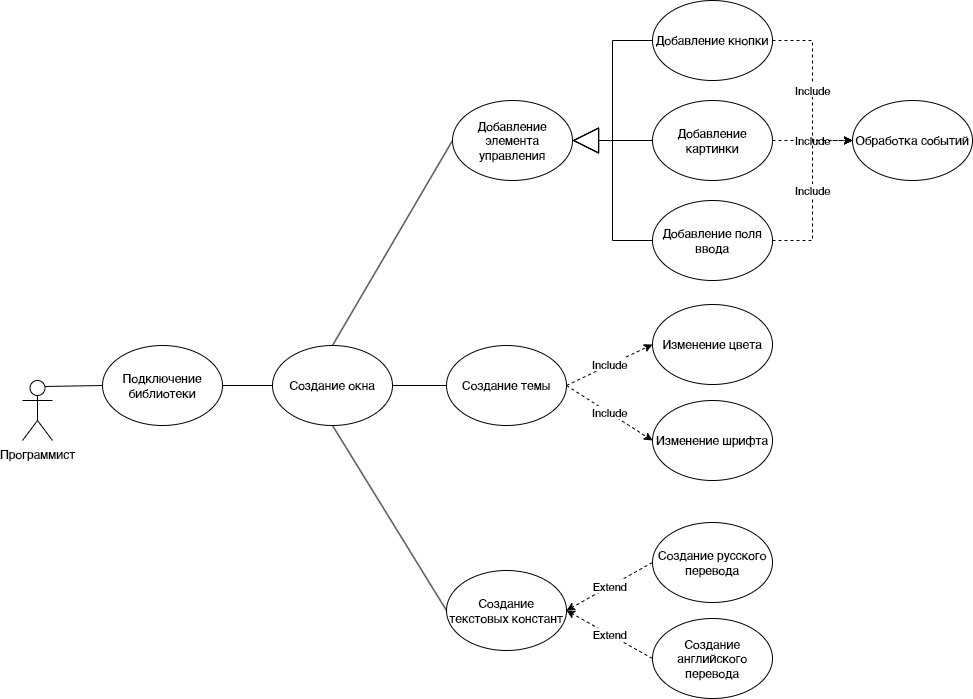
\includegraphics[width=1\linewidth]{use}
	\caption{Варианты использования фреймворка}
	\label{use:image}
\end{figure}

\subsubsection{Вариант использлвания "<Добавление изображения">}
Заинтересованные лица и их требования: пользователь желает добавить изображение.
Предусловие: пользователь создал папку images в папке res и создал нужные темы.
Постусловие: Изображение повилось в окне.

Основной успешный сценарий:
\begin{enumerate}
	\item Пользователь создал несколько вариантов изображений.
	\item Пользователь включил изображения в реестр.
	\item Пользователь добавил переменную изображения и приписал к ней реестр в файле заголовка.
	\item Пользователь прописал название ресурса и путь к изображению в файле ресурсов.
	\item Пользователь прописал изображение в файле темы.
	\item Пользователь добавил элемент управления с помощью метода add{\_}control() в коде.
	\item Пользователь прописал позицию в методе UpdateControlsPosition().
\end{enumerate}

\subsubsection{Вариант использлвания "<Добавление кнопки">}
Заинтересованные лица и их требования: пользователь желает добавить кнопку.
Предусловие: пользователь создал файл окна и файл темы.
Постусловие: создается ini файл в корневой папке проекта.

Основной успешный сценарий:
\begin{enumerate}
	\item Пользователь добавил переменную кнопки в файле заголовка.
	\item Пользователь прописал событие и связал его с помощью команды bind().
	\item Пользователь создал элемент управления с помощью метода add{\_}control() в коде.
	\item Пользователь прописал позицию в методе UpdateControlsPosition().
	\item Пользователь прописал кнопку в json-файле темы.
\end{enumerate}

\subsubsection{Вариант использлвания "<Создание темы">}
Заинтересованные лица и их требования: пользователь желает создать тему для своего проекта.
Предусловие: пользователь создал json-файл в папке res.
Постусловие: при нажатии кнопки сменяется тема.

Основной успешный сценарий:
\begin{enumerate}
	\item Пользователь создал несколько вариантов тем.
	\item Пользователь прописал название тем в реестре файла "<resources.h">.
	\item Пользователь прописал тип ресурса и путь к темам в файле формата "<.rc">.
	\item Пользователь добавил темы в методе set{\_}app{\_}themes() в файле "<main.cpp">.
	\item Пользователь выбрал первичную тему с помошью config.
	\item Пользователь создал элемент управления switch{\_}theme{\_}button.
\end{enumerate}

\subsubsection{Вариант использлвания "<Создание функции смены языка">}
Заинтересованные лица и их требования: пользователь желает создать файл для быстрой настройки окна и других переменных.
Предусловие: пользователь ввел команду создания файла конфигураций.
Постусловие: при нажатии на кнопку меняется язык.

Основной успешный сценарий:
\begin{enumerate}
	\item Пользователь создал несколько вариантов языка.
	\item Пользователь прописал название языка в реестре файла "<resources.h">.
	\item Пользователь прописал тип ресурса и путь к темам в файле формата "<.rc">.
	\item Пользователь добавил темы в методе set{\_}app{\_}locales() в файле "<main.cpp">.
	\item Пользователь выбрал первичную тему с помошью config.
	\item Пользователь создал элемент управления switch{\_}lang{\_}button.
	\item Пользователь связал язык с нужными элементами.
\end{enumerate}

\subsubsection{Требования к интерфейсу}
Фреймворк должен:
\begin{enumerate}
	\item Обеспечивать создание новых компонентов.
	\item Предоставлять общий интерфейс к подсистеме рисования.
	\item Предоставлять общий интерфейс к событиям. Любой компонент или пользователь может подписаться на любую группу сообщений, в том числе пользовательскую, с возможностью асинхронной отправки/получения сообщений.
	\item Принимать системные сообщения, реагировать на мышь, клавиатуру и прочие события.
	\item Открывать окна и отображать на них компоненты.
    \item Предоставлять систему текстовых констант для заголовков и надписей в зависимости от выбранного языка.
    \item Предоставлять систему тем для изменения шрифтов и цветовых акцентов в зависимости от выбранной темы.
\end{enumerate}

Модель простого окна представлена на рисунке ~\ref{window:image}.

\begin{figure}[ht]
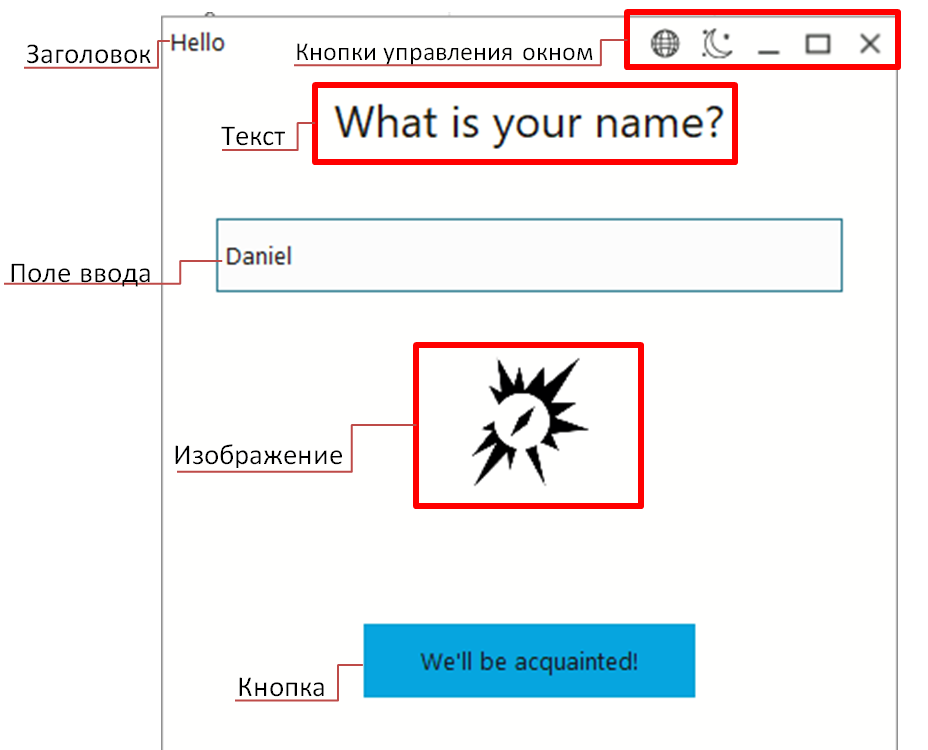
\includegraphics[width=1\linewidth]{window}
\caption{Общая схема простого окна}
\label{window:image}
\end{figure}
%\vspace{-\figureaboveskip} % двойной отступ не нужен (можно использовать, если раздел заканчивается картинкой)

В состав данного окна входят название программы, кнопки управления окном, такие как: кнопка смены темы, кнопка смены языка, кнопка свернуть окно, кнопка развернуть окно, кнопка закрыть окно, и другие элементы взаимодействия, такие как: поле для ввода текста, кнопка подтверждения ввода, различные изображения и текст.

\subsection{Нефункциональные требования к программной системе}

\subsubsection{Требования к надежности}
Приложение должно функционировать на всех разработанных тестах. Тесты требуется разработать на этапе рабочего проекта.
Приложение должено устойчиво функционировать при соблюдении гарантии устойчивого функционирования операционной системы. Под устойчивой работой ПК понимается непрерывное функционирование программы в отсутствии критических сбоев, приводящих к аварийному завершению.

\subsubsection{Требования к аппаратному обеспечению}

Для работы c фреймворком необходимо дисковое пространство не менее 38 Мб, свободная оперативная память в размере не менее 512 Мб, видеокарта с не менее 256 Мб видеопамяти, разрешение экрана не менее 1024*768, клавиатура, мышь.

\subsection{Требования к оформлению документации}

Требования к стадиям разработки программ и программной документации для вычислительных машин, комплексов и систем независимо от их назначения и области применения, этапам и содержанию работ устанавливаются ГОСТ 19.102–77.

Программная документация должна включать в себя:
\begin{enumerate}
	\item Анализ предметной области.
	\item Техническое задание.
	\item Технический проект.
	\item Рабочий проект.
\end{enumerate}

\section{Технический проект}
\subsection{Общая характеристика организации решения задачи}

Необходимо спроектировать и разработать фреймворк, который должен ускорить разработку графических интерфейсов и оптимизировать емкостные характеристики приложения.
Основое внимание следует уделить самым важным элементам взаимодействия с пользователем и выполняемого ими функционала.

\subsubsection{Обоснование выбора технологии проектирования}

На сегодняшний день информационный рынок, поставляющий программные решения в выбранной сфере, предлагает множество продуктов, позволяющих достигнуть поставленной цели – создание фреймворка.
В процессе разработки фреймворка используются язык программирования С++. Также, значения основных переменных задавались в json-файлах.

\subsubsection{Язык программирования С++}

С++ – это высокоуровневый язык программирования общего назначения. Этот язык программирования зарекомендовал себя, ибо уже имеет множество библиотек и фреймворков.

Преимущества использования языка C++ при создании фреймворков:
\begin{enumerate}
\item Высокая производительность: C++ является компилируемым языком с низким уровнем абстракции, что позволяет создавать быстрые и эффективные фреймворки.
\item Возможность доступа к аппаратному обеспечению: C++ позволяет напрямую управлять памятью и ресурсами компьютера, что полезно при разработке фреймворков, работающих с аппаратным обеспечением.
\item Богатая функциональность: C++ обладает множеством возможностей и библиотек, что позволяет создавать мощные и гибкие фреймворки для различных целей.
\end{enumerate}

Недостатки использования языка C++ при создании фреймворков:
\begin{enumerate}
\item Сложность: C++ – сложный и мощный язык программирования, который требует от разработчиков высокого уровня квалификации. Это может затруднить разработку и поддержку фреймворка, особенно для менее опытных программистов.
\item Низкая гибкость: Использование C++ может привести к более жесткой архитектуре фреймворка, что может затруднить его дальнейшее развитие и модификацию.
\item Сильная типизация: C++ имеет сильную статическую типизацию, что может потребовать более тщательного и длительного процесса разработки, особенно при работе с большими проектами.
\end{enumerate}

Таким образом, использование языка С++ при разработке фреймворков обладает рядом преимуществ. Во-первых, С++ является высокопроизводительным языком программирования, что позволяет создавать быстрые и эффективные фреймворки. Во-вторых, С++ обладает богатыми возможностями для объектно-ориентированного программирования, что упрощает создание модульной и расширяемой архитектуры фреймворка. Кроме того, С++ поддерживает многопоточность, что позволяет улучшить производительность и масштабируемость фреймворка. В целом, использование языка С++ при разработке фреймворков позволяет создавать мощные, гибкие и эффективные инструменты для разработки программного обеспечения.

\subsubsection{Cравнение методов отрисовки компонетов}

GDI+ (Graphics Device Interface+) - это набор API для отрисовки 2D графики в операционной системе Windows. Он предоставляет набор простых методов для рисования примитивов, текста, изображений и других графических элементов. GDI+ поддерживает аппаратное ускорение графики и имеет удобный интерфейс для работы с изображениями. Однако он ограничен в возможностях 3D графики.

OpenGL\cite{gl} - это кросс-платформенная библиотека для отображения 2D и 3D графики. Она предоставляет низкоуровневый доступ к графическому аппарату компьютера и поддерживает широкий спектр возможностей, включая шейдеры, текстурирование, освещение и другие эффекты. OpenGL позволяет создавать более сложные и реалистичные графические эффекты, чем GDI+, но требует более глубокого понимания работы с графикой.

Vulkan\cite{vulkan} - это новое поколение библиотеки для написания графических приложений, разработанное компанией Khronos Group. Она предоставляет низкоуровневый доступ к графическому аппарату и позволяет максимально эффективно использовать мощности современных GPU. Vulkan обеспечивает высокую производительность и позволяет параллельно обрабатывать большое количество графических команд. Однако для работы с ней требуется глубокое знание графического программирования.

При создании графических интерфейсов для приложений можно использовать любой из указанных методов в зависимости от требуемого уровня сложности и производительности. GDI+ подходит для простых 2D интерфейсов, OpenGL позволяет создавать более сложные 2D и 3D графику, а Vulkan обеспечивает высокую производительность и возможности для создания сложных 3D интерфейсов. Из-за своей простоты я выбрал Graphics Device Interface+.

\subsubsection{Достоинства Json}

JSON (JavaScript Object Notation) - это легкий формат обмена данными, основанный на тексте, который используется для передачи структурированных данных между программами.

Преимущества JSON:
\begin{enumerate}
\item Простота использования: JSON легко читаем и понятен людям, что делает его удобным для работы с данными.
\item Легкость: JSON файлы компактны и занимают мало места, что ускоряет передачу данных и уменьшает нагрузку на сеть.
\item Поддержка множества языков программирования: JSON поддерживается большинством языков программирования, что делает его универсальным форматом для обмена данными между различными системами.
\item Поддержка структурированных данных: JSON поддерживает различные типы данных, включая строки, числа, логические значения, массивы и объекты, что позволяет передавать сложные структуры данных.
\item Гибкость: JSON позволяет легко добавлять, изменять и удалять данные, а также манипулировать ими, что делает его удобным для работы с динамическими данными.
\end{enumerate}
Таким образом, использование JSON упрощает обмен данными между различными системами и позволяет эффективно передавать информацию в формате, который легко читать и понять.

\subsection{Диаграмма компонентов и схема обмена данными между классами}

Диаграмма компонентов описывает особенности физического представления разрабатываемой системы. Она позволяет определить архитектуру системы, установив зависимости между программными компонентами, в роли которых может выступать как исходный, так и исполняемый код. Основными графическими элементами диаграммы компонентов являются классы, а также зависимости между ними. На рисунке \ref{comp:image} изображена диаграмма компонентов для проектируемой системы. Она базируется на двух сущностях - Window и Control. Окно может содержать контролы, также само окно является контролом.

\begin{figure}[H]
\center{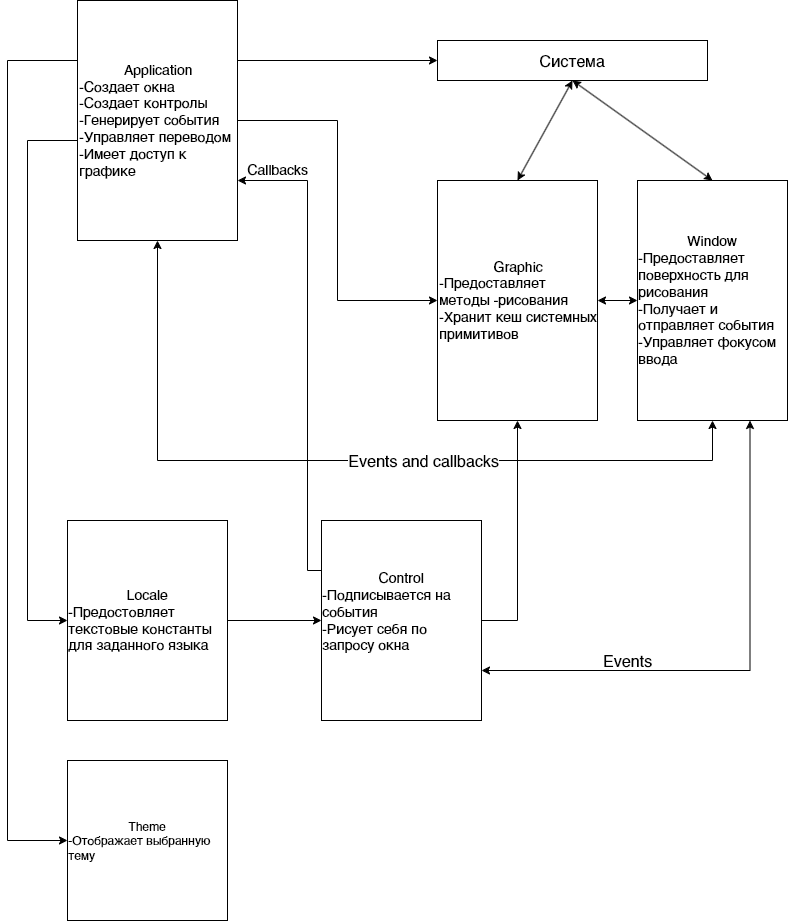
\includegraphics[width=1\linewidth]{comp}}
\caption{Cхема обмена данными между классами}
\label{comp:image}
\end{figure}

\subsection{Описание основных сущностей}

Проанализировав требования, можно выделить девять основных сущностей:
\begin{enumerate}
\item "<Фреймворк">.
\item "<Окно">.
\item "<Компонент">.
\item "<Кнопка">.
\item "<Изображение">.
\item "<Графика">.
\item "<Тема">.
\item "<Локаль">.
\item "<Ошибка">.
\end{enumerate}

В состав сущности "<Фреймворк"> можно включить атрибуты, представленные в таблице \ref{framework_a:table}.

\begin{xltabular}{\textwidth}{|l|l|p{1.7cm}|X|}
	\caption{Атрибуты сущности "<Фреймворк">\label{framework_a:table}}\\ \hline
	\centrow Поле & \centrow Тип & \centrow Обяза\-тельное & \centrow Описание \\ \hline
	\thead{1} & \thead{2} & \centrow 3 & \centrow 4 \\ \hline
	\endfirsthead
	\continuecaption{Продолжение таблицы \ref{framework_a:table}}
	\thead{1} & \thead{2} & \centrow 3 & \centrow 4 \\ \hline
	\finishhead
	\ runned & bool & false & Флаг запуска приложения \\ \hline
	err & error & false & Ошибка
\end{xltabular}

В состав сущности "<Ошибка"> можно включить атрибуты, представленные в таблице \ref{error_a:table}.

\begin{xltabular}{\textwidth}{|l|l|p{1.7cm}|X|}
	\caption{Атрибуты сущности "<Ошибка">\label{error_a:table}}\\ \hline
	\centrow Поле & \centrow Тип & \centrow Обяза\-тельное & \centrow Описание \\ \hline
	\thead{1} & \thead{2} & \centrow 3 & \centrow 4 \\ \hline
	\endfirsthead
	\continuecaption{Продолжение таблицы \ref{error_a:table}}
	\thead{1} & \thead{2} & \centrow 3 & \centrow 4 \\ \hline
	\finishhead
	\ type & error{\_}type & true & тип ошибки \\ \hline
	component & string & true & указатель на компонент, вызвавший ошибку \\ \hline
	message & string & true & Сообщение \\ \hline
\end{xltabular}

В состав сущности "<Графика"> можно включить атрибуты, представленные в таблице \ref{graphic_a:table}.

\begin{xltabular}{\textwidth}{|l|l|p{1.7cm}|X|}
	\caption{Атрибуты сущности "<Графика">\label{graphic_a:table}}\\ \hline
	\centrow Поле & \centrow Тип & \centrow Обяза\-тельное & \centrow Описание \\ \hline
	\thead{1} & \thead{2} & \centrow 3 & \centrow 4 \\ \hline
	\endfirsthead
	\continuecaption{Продолжение таблицы \ref{graphic_a:table}}
	\thead{1} & \thead{2} & \centrow 3 & \centrow 4 \\ \hline
	\finishhead
	\ pc & primitive{\_}container & true & Примитивный контейнер для хранения \\ \hline
	max{\_}size & rect & true & максимальный размер \\ \hline
	background{\_}color & color & true & Задний фон \\ \hline
	mem{\_}dc & HDC & true & Указатель на графический объект \\ \hline
	mem{\_}bitmap & HBITMAP & true & Указатель на битмап \\ \hline
	err & error & false & Ошибка
\end{xltabular}

В состав сущности "<Компонент"> можно включить атрибуты, представленные в таблице \ref{control_a:table}.

\begin{xltabular}{\textwidth}{|l|l|p{1.7cm}|X|}
	\caption{Атрибуты сущности "<Компонент">\label{control_a:table}}\\ \hline
	\centrow Поле & \centrow Тип & \centrow Обяза\-тельное & \centrow Описание \\ \hline
	\thead{1} & \thead{2} & \centrow 3 & \centrow 4 \\ \hline
	\endfirsthead
	\continuecaption{Продолжение таблицы \ref{control_a:table}}
	\thead{1} & \thead{2} & \centrow 3 & \centrow 4 \\ \hline
	\finishhead
	\_position & rect & true & Позиция элемента \\ \hline
	parent & window & true & Родительское окно \\ \hline 
	topmost & bool & true & Флаг "<Поверх всех элементов"> \\ \hline 
	showed & bool & true & Видимость элемента \\ \hline 
	enabled & bool & true & Включенность элемента \\ \hline 
	focused & bool & false & Возвращает true, если элемент управления сфокусирован \\ \hline 
	focusing & bool & false & Возвращает true, если элемент управления получает фокус \\ \hline
	err & error & false & Ошибка
\end{xltabular}

В состав сущности "<Компонент Кнопка"> можно включить атрибуты, представленные в таблице \ref{button_a:table}.

\begin{xltabular}{\textwidth}{|l|l|p{1.7cm}|X|}
	\caption{Атрибуты сущности "<Кнопка">\label{button_a:table}}\\ \hline
	\centrow Поле & \centrow Тип & \centrow Обяза\-тельное & \centrow Описание \\ \hline
	\thead{1} & \thead{2} & \centrow 3 & \centrow 4 \\ \hline
	\endfirsthead
	\continuecaption{Продолжение таблицы \ref{button_a:table}}
	\thead{1} & \thead{2} & \centrow 3 & \centrow 4 \\ \hline
	\finishhead
	\ button{\_}view{\_} & button{\_}view & true & Вид кнопки \\ \hline
	caption & string & true & Надпись на кнопке \\ \hline
	image{\_} & string & false & Изображение на кнопке \\ \hline
	image{\_}size & int32{\_}t & false & Размер изображения \\ \hline
	tooltip{\_} & tooltip & false & Подсказка при наведения на кнопку \\ \hline
	theme{\_}  & i{\_}theme & true & Тема кнопки \\ \hline
	{\_}position & rect & true & Позиция элемента \\ \hline
	parent & window & true & Родительское окно \\ \hline
	my{\_}subscriber{\_}id & string & true & Подписка на события \\ \hline
	topmost & bool & true & Флаг "<Поверх всех элементов"> \\ \hline 
	pushed, turned & bool & false & Флаг "<Включения кнопки"> \\ \hline 
	showed & bool & true & Видимость элемента \\ \hline 
	enabled & bool & true & Включенность \\ \hline 
	focused & bool & false & Возвращает true, если элемент управления сфокусирован \\ \hline 
	focusing & bool & false & Возвращает true, если элемент управления получает фокус \\ \hline
	err & error & false & Ошибка
\end{xltabular}

В состав сущности "<Компонент Изображение"> можно включить атрибуты, представленные в таблице \ref{img_a:table}.

\begin{xltabular}{\textwidth}{|l|l|p{1.7cm}|X|}
	\caption{Атрибуты сущности "<Изображение">\label{img_a:table}}\\ \hline
	\centrow Поле & \centrow Тип & \centrow Обяза\-тельное & \centrow Описание \\ \hline
	\thead{1} & \thead{2} & \centrow 3 & \centrow 4 \\ \hline
	\endfirsthead
	\continuecaption{Продолжение таблицы \ref{img_a:table}}
	\thead{1} & \thead{2} & \centrow 3 & \centrow 4 \\ \hline
	\finishhead
	\ img{\_} & Gdiplus::Image & true & Полотно изображения \\ \hline
	file{\_}name & string & true & Имя изображения \\ \hline
	resource{\_}index & int32{\_}t & true & Индекс ресурса \\ \hline
	theme{\_}  & i{\_}theme & true & Тема изображения \\ \hline
	{\_}position & rect & true & Позиция изображения \\ \hline
	parent & window & true & Родительское окно \\ \hline
	topmost & bool & true & Флаг "<Поверх всех элементов"> \\ \hline 
	showed & bool & true & Видимость элемента \\ \hline  
	err & error & false & Ошибка
\end{xltabular}

В состав сущности "<Окно"> можно включить атрибуты, представленные в таблице \ref{window_a:table}.

\begin{xltabular}{\textwidth}{|l|l|p{1.7cm}|X|}
	\caption{Атрибуты сущности "<Окно">\label{window_a:table}}\\ \hline
	\centrow Поле & \centrow Тип & \centrow Обяза\-тельное & \centrow Описание \\ \hline
	\thead{1} & \thead{2} & \centrow 3 & \centrow 4 \\ \hline
	\endfirsthead
	\continuecaption{Продолжение таблицы \ref{window_a:table}}
	\thead{1} & \thead{2} & \centrow 3 & \centrow 4 \\ \hline
	\finishhead
	\ graphic{\_} & rect & true & Полотно для рисования \\ \hline
	controls & std::vector & true & Компоненты окна \\ \hline
	active{\_}control & i{\_}control & true & Активный компонент \\ \hline
	caption & string & true & Название окна \\ \hline
	{\_}position, normal{\_}position & rect & true & Позиция окна \\ \hline
	min{\_}width, min{\_}height & int32{\_}t & true & Минимальная высота/ширина окна \\ \hline
	window{\_}style{\_} &  window{\_}style & true & Тип окна \\ \hline
	window{\_}state{\_}, prev{\_}window{\_}state{\_} & window{\_}state & true & Состояние окна \\ \hline
	theme{\_} & i{\_}theme & true & Тема окна \\ \hline
	showed & bool & true & Видимость окна \\ \hline  
	skip{\_}draw{\_} & bool & true & Флаг пропуска отрисовки \\ \hline
	focused & bool & false & Фокус\\ \hline 
	docked{\_} & bool & false & Флаг прикрепления к окну \\ \hline 
	docked{\_}control & i{\_}control & false & Прикреп-\ ленный к окну элемент \\ \hline 
	subscribers{\_} & std::vector & false & Подписанные на события элементы \\ \hline
	mouse{\_}tracked & bool & false & Флаг отслеживания мыши \\ \hline
	x{\_}click, y{\_}click & int16{\_}t & false & Координаты клика \\ \hline 
	switch{\_}lang{\_}button & button & true & Кнопка управления языком \\ \hline
	switch{\_}theme{\_}button & button & true & Кнопка управления темой \\ \hline
	pin{\_}button & button & true & Кнопка управления закреплением \\ \hline
	minimize{\_}button & button & true & Кнопка "<Свернуть"> \\ \hline
	expand{\_}button & button & true & Кнопка "<Расширить"> \\ \hline
	close{\_}button & button & true & Кнопка "<Закрыть"> \\ \hline
	err & error & false & Ошибка
\end{xltabular}

В состав сущности "<Локаль"> можно включить атрибуты, представленные в таблице \ref{locale_a:table}.

\begin{xltabular}{\textwidth}{|l|l|p{1.7cm}|X|}
	\caption{Атрибуты сущности "<Локаль">\label{locale_a:table}}\\ \hline
	\centrow Поле & \centrow Тип & \centrow Обяза\-тельное & \centrow Описание \\ \hline
	\thead{1} & \thead{2} & \centrow 3 & \centrow 4 \\ \hline
	\endfirsthead
	\continuecaption{Продолжение таблицы \ref{locale_a:table}}
	\thead{1} & \thead{2} & \centrow 3 & \centrow 4 \\ \hline
	\finishhead
	\ type & locale{\_}type & true & Код языка\\ \hline
	name & string & true & Название \\ \hline 
	strings & std::map & true & Строки перевода \\ \hline 
	dummy{\_}string & string & true & Строка по умолчанию \\ \hline 
	err & error & false & Ошибка
\end{xltabular}

В состав сущности "<Тема"> можно включить атрибуты, представленные в таблице \ref{theme_a:table}.

\begin{xltabular}{\textwidth}{|l|l|p{1.7cm}|X|}
	\caption{Атрибуты сущности "<Тема">\label{theme_a:table}}\\ \hline
	\centrow Поле & \centrow Тип & \centrow Обяза\-тельное & \centrow Описание \\ \hline
	\thead{1} & \thead{2} & \centrow 3 & \centrow 4 \\ \hline
	\endfirsthead
	\continuecaption{Продолжение таблицы \ref{theme_a:table}}
	\thead{1} & \thead{2} & \centrow 3 & \centrow 4 \\ \hline
	\finishhead
	\ type & locale{\_}type & true & Код языка\\ \hline
	name & string & true & Название \\ \hline 
	ints & std::map & true & Коллекция чисел \\ \hline
	strings & std::map & true & Строки \\ \hline
	fonts & std::map & true & Коллекция шрифтов \\ \hline
	imgs & std::map & true & Коллекция изображений \\ \hline
	dummy{\_}string & string & true & Строка по умолчанию \\ \hline
	dummy{\_}image & std::vector<uint8{\_}t> & true & Изображение по умолчанию \\ \hline 
	err & error & false & Ошибка
\end{xltabular}

В системе предусмотрен внутренний механизм связи между разделами и элементами информационных блоков, поэтому введения дополнительных идентификаторов при реализации связей между сущностями не предполагается.

Экземпляры сущностей реализуются в информационных блоках посредством элементов, атрибуты сущности – посредством полей и свойств элемента. 

\subsection{Описание сущностей для настройки окна}

В состав сущности "<Тема"> можно включить набор основных полей JSON-документа и их описание, представленные в таблице \ref{json-theme:table}.


\begin{xltabular}{\textwidth}{|X|>{\setlength{\baselineskip}{0.7\baselineskip}}p{4.85cm}|>{\setlength{\baselineskip}{0.7\baselineskip}}p{4.85cm}|}
	\caption{Описание полей JSON-документа сущности "<Тема">\label{json-theme:table}}\\
	\hline \centrow \setlength{\baselineskip}{0.7\baselineskip} Ключ & \centrow Тип & \centrow Описание \\
	\hline \centrow 1 & \centrow 2 & \centrow 3 \\ \hline
	\endfirsthead
	\caption*{Продолжение таблицы \ref{json-theme:table}}\\
	\hline \centrow 1 & \centrow 2 & \centrow 3 \\ \hline
	\finishhead
	controls & map & Элементы управления \\ \hline
	type & str & Тип элемента управления \\ \hline
	background & str & Цвет заднего фона \\ \hline
	border & str & Цвет обводки  \\ \hline
	border{\_}width & number & Ширина обводки \\ \hline
	round & number & Округление \\ \hline
	text & str & Цвет текста \\ \hline
	caption{\_}font & map & Шрифт заголовка \\ \hline
	name & str & Название шрифта \\ \hline
	size & number & Размер шрифта \\ \hline
	color & str & Цвет заливки \\ \hline
	resource & str & Название ресурса \\ \hline
	path & str & Путь к папке \\ \hline
	calm & str & Основной цвет \\ \hline
	active & str & Активный цвет \\ \hline
	focused{\_}border & str & Цвет обводки при фокусировке \\ \hline
	disabled & str & Цвет при недоступности \\ \hline
	anchor & str & Цвет ссылки \\ \hline
	focusing & number & фокусировка \\ \hline
	selection & str & Цвет при выборе поля ввода \\ \hline
	button{\_}calm & str & Основной цвет кпонки при выборе клавиатурой \\ \hline
	button{\_}active & str & Цвет активированной кнопки при выборе клавиатурой \\ \hline
	scrollbar & str & Цвет полосы прокрутки \\ \hline
	scrollbar{\_}slider & str & Цвет ползунка полосы прокрутки \\ \hline
	scrollbar{\_}slider{\_}active & str & Цвет активного ползунка полосы прокрутки \\ \hline
	selected{\_}item & str & Цвет выбранного элемента \\ \hline
	active{\_}item & str & Цвет активного элемента \\ \hline
	title & str & Цвет заголовка листа \\ \hline
	title{\_}text & str & Цвет текста заголовка листа \\ \hline
	slider & str & Цвет ползунка \\ \hline
	slider{\_}active & str & Цвет активного ползунка \\ \hline
	disabled{\_}text & str & Цвет неактивного текста в меню \\ \hline
	text{\_}indent & number & Отступ текста \\ \hline
	meter & str & Цвет полосы прогресса \\ \hline
	perform & str & Цвет активной части ползунка настройки \\ \hline
	remain & str & Цвет неактивной части ползунка настройки  \\ \hline
	slider{\_}width & number & Ширина ползунка настройки \\ \hline
	slider{\_}height & number & Высота ползунка настройки \\ \hline
	images & map & Иконки окна
\end{xltabular}

В состав сущности "<Язык"> можно включить набор основных полей JSON-документа и их описание, представленные в таблице \ref{json-locale:table}.


\begin{xltabular}{\textwidth}{|X|>{\setlength{\baselineskip}{0.7\baselineskip}}p{4.85cm}|>{\setlength{\baselineskip}{0.7\baselineskip}}p{4.85cm}|}
	\caption{Описание полей JSON-документа сущности "<Тема">\label{json-locale:table}}\\
	\hline \centrow \setlength{\baselineskip}{0.7\baselineskip} Ключ & \centrow Тип & \centrow Описание \\
	\hline \centrow 1 & \centrow 2 & \centrow 3 \\ \hline
	\endfirsthead
	\caption*{Продолжение таблицы \ref{json-locale:table}}\\
	\hline \centrow 1 & \centrow 2 & \centrow 3 \\ \hline
	\finishhead
	sections & map & Элементы управления \\ \hline
	type & str & Тип элемента управления \\ \hline
	ok & str & Подтверждение \\ \hline
	yes & str & Да  \\ \hline
	no & str & Нет \\ \hline
	cancel & number & Отмена \\ \hline
	abort & str & Отказ \\ \hline
	retry & str & Повторить \\ \hline
	ignore & str & Пропустить \\ \hline
	try{\_}continue & str & Попробовать продолжить \\ \hline
	complete & str & Готово \\ \hline
	pin & str & Прикрепить окно \\ \hline
	unpin & str & Открепить окно \\ \hline
	dark{\_}theme & str & Темная тема \\ \hline
	light{\_}theme & str & Светлая тема\\ \hline
	switch{\_}lang & str & Сменить язык \\ \hline
	copy & str & Копировать \\ \hline
	cut & str & Вырезать \\ \hline
	paste & number & Вставить \\ \hline
	undo & str & Отменить \\ \hline
	redo & str & Вернуть отмену
\end{xltabular}

\ifПрактика{}\else{
   \section{Рабочий проект}
\subsection{Спецификация классов фреймворка}

Класс Framework инициализирует фреймфорк. Запускает GDI+. Запускает или останавливает работу. (таблица \ref{framework_m:table}).

\renewcommand{\arraystretch}{0.8} % уменьшение расстояний до сетки таблицы
\begin{xltabular}{\textwidth}{|X|>{\setlength{\baselineskip}{0.7\baselineskip}}p{4.85cm}|>{\setlength{\baselineskip}{0.7\baselineskip}}p{4.85cm}|}
	\caption{Спецификация методов класса Framework\label{framework_m:table}}\\
	\hline \centrow \setlength{\baselineskip}{0.7\baselineskip} Название & \centrow Метод дрступа & \centrow Описание \\
	\hline \centrow 1 & \centrow 2 & \centrow 3 \\ \hline
	\endfirsthead
	\continuecaption{Продолжение таблицы \ref{framework_m:table}}
	\hline \centrow 1 & \centrow 2 & \centrow 3 \\ \hline
	\finishhead
	init & public & Запуск GDI+ \\ \hline
	run & public & Запускает приложение \\ \hline
	stop & public & Останавливает работу приложения
\end{xltabular}
\renewcommand{\arraystretch}{1.0} % восстановление сетки

Класс Window создает окна для приложения. Принимает системные события и обеспечивает их рассылку подписчикам. Так же окно дает команду на перерисовку своих компонентов и предоставляет им свой graphic. Кроме этого, окно управляет фокусом ввода, может сделать модальность и отправить подписанному пользователю или в систему событие. (таблица \ref{window_m:table}).

\renewcommand{\arraystretch}{0.8} % уменьшение расстояний до сетки таблицы
\begin{xltabular}{\textwidth}{|X|>{\setlength{\baselineskip}{0.7\baselineskip}}p{4.85cm}|>{\setlength{\baselineskip}{0.7\baselineskip}}p{4.85cm}|}
	\caption{Спецификация методов класса Window\label{window_m:table}}\\
	\hline \centrow \setlength{\baselineskip}{0.7\baselineskip} Название & \centrow Метод дрступа & \centrow Описание \\
	\hline \centrow 1 & \centrow 2 & \centrow 3 \\ \hline
	\endfirsthead
	\continuecaption{Продолжение таблицы \ref{window_m:table}}
	\hline \centrow 1 & \centrow 2 & \centrow 3 \\ \hline
	\finishhead
	init & public & Создание окна \\ \hline
	destroy & public & Уничтожение  окна \\ \hline
	add{\_}control & public & Добавление контрола \\ \hline
	remove{\_}control & public & Удаление контрола \\ \hline
	bring{\_}to{\_}front, move{\_}to{\_}back & public & Изменеие порядка слоев элементов \\ \hline
	set{\_}position & public & Изменеие позиции окна \\ \hline
	position & public & Возвращение позиции окна \\ \hline
	set{\_}parent & public & Установление родительского окна \\ \hline
	parent & public & Возвращение родительского окна \\ \hline
	clear{\_}parent & public & Очищение свойства родительского окна \\ \hline
	update{\_}theme & public & Обновление темы \\ \hline
	redraw & public & Перерисовывает часть окна. Вызывается компонентом окна. \\ \hline
	subscribe & public & Подписка на события \\ \hline
	unsubscribe & public & Отписка от событий \\ \hline
	emit{\_}event & public & Посылает сообщение через системный шедулер сообщений \\ \hline
	set{\_}caption & public & Изменяет название окна \\ \hline
	set{\_}style & public & Изменяет стиль окна \\ \hline
	set{\_}min{\_}size & public & Изменяет минимальный размер окна \\ \hline
	switch{\_}lang & public & Изменяет язык  \\ \hline
	switch{\_}theme & public & Изменяет тему  \\ \hline
	pin & public & Прикрепляет окно \\ \hline
	minimize & public & Сворачивает окно \\ \hline
	expand & public & Расширяет окно \\ \hline
	normal & public & Возвращает окно в исходное состояние \\ \hline
	state & public & Изменяет состояние окна \\ \hline
	disable{\_}draw, enable{\_}draw& public & Отключает/Включает рисование для повышения производительности при выполнении массовых операций \\ \hline
	set{\_}focused & public & Делает компонент окна сфокусированным \\ \hline
	set{\_}control{\_}callback & public & Привязывает событие к компоненту \\ \hline
	set{\_}default{\_}push{\_}control & public & Нажатие кнопки по клавише Enter \\ \hline
	receive{\_}control{\_}events & private & Принимает события от компонентов \\ \hline
	send{\_}event{\_}to{\_}control & private & Посылает событие компоненту \\ \hline
	send{\_}mouse{\_}event & private & Посылает событие мыши \\ \hline
	check{\_}control{\_}here & private & Проверяет компонент на месте клика \\ \hline
	change{\_}focus & private & Изменяет фокус \\ \hline
	get{\_}focused & private & Возвращает сфокусированый элемент \\ \hline
	start{\_}docking, end{\_}docking & private & Включает/отключает привязку к окну \\ \hline
	draw{\_}border & private & Рисукет границы графического контекста \\ \hline
	send{\_}system & private & Отправить системное сообщение
\end{xltabular}
\renewcommand{\arraystretch}{1.0} % восстановление сетки

Класс Control - это любой визуальный элемент для взаимодействия с пользователем - кнопка, поле ввода, список, меню и т.д. Control знает, как обрабатывать события, поступающие от Window, хранит свои состояния и рисует себя на графическом контексте, который предоставляется содержащим его окном. (таблица \ref{control_m:table}).

\renewcommand{\arraystretch}{0.8} % уменьшение расстояний до сетки таблицы
\begin{xltabular}{\textwidth}{|X|>{\setlength{\baselineskip}{0.7\baselineskip}}p{4.85cm}|>{\setlength{\baselineskip}{0.7\baselineskip}}p{4.85cm}|}
	\caption{Спецификация методов класса Сontrol\label{control_m:table}}\\
	\hline \centrow \setlength{\baselineskip}{0.7\baselineskip} Название & \centrow Метод дрступа & \centrow Описание \\
	\hline \centrow 1 & \centrow 2 & \centrow 3 \\ \hline
	\endfirsthead
	\continuecaption{Продолжение таблицы \ref{control_m:table}}
	\hline \centrow 1 & \centrow 2 & \centrow 3 \\ \hline
	\finishhead
	draw & public & Рисует компонент. Вызывается окном. \\ \hline
	set{\_}position & public & Изменяет положение контрола на окне. Координаты задаются в пикселях относительно левого верхнего угла родительского окна.  \\ \hline
	position & public & Возвращает положение контрола относительно окна \\ \hline
	set{\_}parent & public & Позволяет контролу получить указатель на свое родительское окно \\ \hline
	parent & public & Возвращает указатель на родительское окно \\ \hline
	clear{\_}parent & public & Очищает указатель на родительское окно контрола \\ \hline
	topmost & public & Сообщает родительскому окну, нужно ли рисовать контрол поверх всех остальных контролов \\ \hline
	update{\_}theme & public & Изменяет визуальную тему контрола \\ \hline
	show,hide,showed & public & Методы управления видимостью \\ \hline
	enable,disable,enabled & public & Методы управления включенностью \\ \hline
	focused,focusing & public & Клавиатурный фокус ввода \\ \hline
	get{\_}error & public & Возвращает структуру, содержащую подробности последней ошибки
\end{xltabular}
\renewcommand{\arraystretch}{1.0} % восстановление сетки

Класс Image создает изображение на экране. (таблица \ref{image_m:table}).

\renewcommand{\arraystretch}{0.8} % уменьшение расстояний до сетки таблицы
\begin{xltabular}{\textwidth}{|X|>{\setlength{\baselineskip}{0.7\baselineskip}}p{4.85cm}|>{\setlength{\baselineskip}{0.7\baselineskip}}p{4.85cm}|}
	\caption{Спецификация методов класса Image\label{image_m:table}}\\
	\hline \centrow \setlength{\baselineskip}{0.7\baselineskip} Название & \centrow Метод дрступа & \centrow Описание \\
	\hline \centrow 1 & \centrow 2 & \centrow 3 \\ \hline
	\endfirsthead
	\continuecaption{Продолжение таблицы \ref{image_m:table}}
	\hline \centrow 1 & \centrow 2 & \centrow 3 \\ \hline
	\finishhead
	image & public & Создает изображение \\ \hline
	change{\_}image & public & Изменяет изображение \\ \hline
	width, height & public & Возвращает ширину/высоту изображения \\ \hline
	draw & public & Рисует изображение. Вызывается окном. \\ \hline
	set{\_}position & public & Изменяет положение контрола на окне. Координаты задаются в пикселях относительно левого верхнего угла родительского окна.  \\ \hline
	position & public & Возвращает положение контрола относительно окна \\ \hline
	set{\_}parent & public & Позволяет контролу получить указатель на свое родительское окно \\ \hline
	parent & public & Возвращает указатель на родительское окно \\ \hline
	clear{\_}parent & public & Очищает указатель на родительское окно контрола \\ \hline
	topmost & public & Сообщает родительскому окну, нужно ли рисовать контрол поверх всех остальных контролов \\ \hline
	update{\_}theme & public & Изменяет визуальную тему контрола \\ \hline
	show,hide,showed & public & Методы управления видимостью \\ \hline
	enable,disable,enabled & public & Методы управления включенностью \\ \hline
	focused,focusing & public & Клавиатурный фокус ввода \\ \hline
	get{\_}error & public & Возвращает структуру, содержащую подробности последней ошибки
\end{xltabular}
\renewcommand{\arraystretch}{1.0} % восстановление сетки

Класс Button - это любая кнопка для взаимодействия с пользователем. Кнопка знает, как обрабатывать события, поступающие от Window, хранит свои состояния и рисует себя на графическом контексте, который предоставляется содержащим его окном. (таблица \ref{button_m:table}).

\renewcommand{\arraystretch}{0.8} % уменьшение расстояний до сетки таблицы
\begin{xltabular}{\textwidth}{|X|>{\setlength{\baselineskip}{0.7\baselineskip}}p{4.85cm}|>{\setlength{\baselineskip}{0.7\baselineskip}}p{4.85cm}|}
	\caption{Спецификация методов класса Button\label{button_m:table}}\\
	\hline \centrow \setlength{\baselineskip}{0.7\baselineskip} Название & \centrow Метод дрступа & \centrow Описание \\
	\hline \centrow 1 & \centrow 2 & \centrow 3 \\ \hline
	\endfirsthead
	\continuecaption{Продолжение таблицы \ref{button_m:table}}
	\hline \centrow 1 & \centrow 2 & \centrow 3 \\ \hline
	\finishhead
	button & public & Функция создания кнопки. \\ \hline
	draw & public & Рисует кнопку. \\ \hline
	set{\_}position & public & Изменяет положение контрола на окне. Координаты задаются в пикселях относительно левого верхнего угла родительского окна.  \\ \hline
	position & public & Возвращает положение контрола относительно окна \\ \hline
	set{\_}parent & public & Позволяет контролу получить указатель на свое родительское окно \\ \hline
	parent & public & Возвращает указатель на родительское окно \\ \hline
	clear{\_}parent & public & Очищает указатель на родительское окно контрола \\ \hline
	topmost & public & Сообщает родительскому окну, нужно ли рисовать контрол поверх всех остальных контролов \\ \hline
	update{\_}theme & public & Изменяет визуальную тему контрола \\ \hline
	show,hide,showed & public & Методы управления видимостью \\ \hline
	enable,disable,enabled & public & Методы управления включенностью \\ \hline
	focused,focusing & public & Клавиатурный фокус ввода \\ \hline
	get{\_}error & public & Возвращает структуру, содержащую подробности последней ошибки\\ \hline
	update{\_}err & private & Обновляет структуру ошибки\\ \hline
	set{\_}caption & private & Устанавливает надпись на кнопке\\ \hline
	set{\_}button{\_}view & private & Изменяет вид кнопки\\ \hline
	set{\_}image & private & Устанавливает изображение на кнопку\\ \hline
	enable{\_}focusing & private & Включает фокус\\ \hline
	disable{\_}focusing & private & Отключает фокус\\ \hline
	turn & private & Включает кнопку\\ \hline
	turned & private & Возвращает флаг включения кнопки\\ \hline
	set{\_}callback & private & Устанавливает функионал кнопки \\ \hline
	receive{\_}event & private & Получение события \\ \hline
	redraw & private & Перерисовывает кнопку
\end{xltabular}  
\renewcommand{\arraystretch}{1.0} % восстановление сетки

Класс Graphic предоставляет интерфейс к системным методам рисования. В настоящий момент, реализовано рисование на Windows GDI/GDI+. (таблица \ref{graphic:table}).

\renewcommand{\arraystretch}{0.8} % уменьшение расстояний до сетки таблицы
\begin{xltabular}{\textwidth}{|X|>{\setlength{\baselineskip}{0.7\baselineskip}}p{4.85cm}|>{\setlength{\baselineskip}{0.7\baselineskip}}p{4.85cm}|}
	\caption{Спецификация методов класса Graphic\label{graphic:table}}\\
	\hline \centrow \setlength{\baselineskip}{0.7\baselineskip} Название & \centrow Метод дрступа & \centrow Описание \\
	\hline \centrow 1 & \centrow 2 & \centrow 3 \\ \hline
	\endfirsthead
	\continuecaption{Продолжение таблицы \ref{graphic:table}}
	\hline \centrow 1 & \centrow 2 & \centrow 3 \\ \hline
	\finishhead
	init & public & Инициализация \\ \hline
	release & public & Деинициализации  \\ \hline
	set{\_}background{\_}color & public & Устанавливает цвет фона \\ \hline
	clear & public & Заливает холст \\ \hline
	flush & public & Отрисовка области на системный графический контекст \\ \hline
	draw{\_}pixel{\_} & public & Рисует точку \\ \hline
	draw{\_}line & public & Рисует линию \\ \hline
	measure{\_}text & public & Измеряет размер текста с выбранным шрифтом \\ \hline
	draw{\_}text & public & Рисует текст \\ \hline
	draw{\_}rect & public & Рисует прямоугольник \\ \hline
	draw{\_}buffer & public & Рисует буфер RGB32 \\ \hline
	draw{\_}graphic & public & Рисует содержимое другого графика
\end{xltabular}
\renewcommand{\arraystretch}{1.0} % восстановление сетки

Класс Locale нужен для смены языка программы. Он загружает текстовые константы, меняет текущий язык, а также загружает json-файл для быстрой настройки. (таблица \ref{locale_m:table}).

\renewcommand{\arraystretch}{0.8} % уменьшение расстояний до сетки таблицы
\begin{xltabular}{\textwidth}{|X|>{\setlength{\baselineskip}{0.7\baselineskip}}p{4.85cm}|>{\setlength{\baselineskip}{0.7\baselineskip}}p{4.85cm}|}
	\caption{Спецификация методов класса Locale\label{locale_m:table}}\\
	\hline \centrow \setlength{\baselineskip}{0.7\baselineskip} Название & \centrow Метод дрступа & \centrow Описание \\
	\hline \centrow 1 & \centrow 2 & \centrow 3 \\ \hline
	\endfirsthead
	\continuecaption{Продолжение таблицы \ref{locale_m:table}}
	\hline \centrow 1 & \centrow 2 & \centrow 3 \\ \hline
	\finishhead
	get{\_}type() & public & Возвращает код языка \\ \hline
	get{\_}name & public & Возвращает название перевода \\ \hline
	set & public & Меняет текущий язык \\ \hline
	get & public & Возвращает данные перевода \\ \hline
	load{\_}resource & public & Загружает ресурсы перевода \\ \hline
	load{\_}json & public & Загружает json-файл перевода \\ \hline
	load{\_}locale & public & Загружает строки перевода
\end{xltabular}
\renewcommand{\arraystretch}{1.0} % восстановление сетки

Класс Theme нужен для изменение цветовых акцентов окна. Он позволяет менять цвета, шрифты, изображение, а также загружать json-файлы для быстрой настройки. (таблица \ref{theme_m:table}).

\renewcommand{\arraystretch}{0.8} % уменьшение расстояний до сетки таблицы
\begin{xltabular}{\textwidth}{|X|>{\setlength{\baselineskip}{0.7\baselineskip}}p{4.85cm}|>{\setlength{\baselineskip}{0.7\baselineskip}}p{4.85cm}|}
	\caption{Спецификация методов класса Theme\label{theme_m:table}}\\
	\hline \centrow \setlength{\baselineskip}{0.7\baselineskip} Название & \centrow Метод дрступа & \centrow Описание \\
	\hline \centrow 1 & \centrow 2 & \centrow 3 \\ \hline
	\endfirsthead
	\continuecaption{Продолжение таблицы \ref{theme_m:table}}
	\hline \centrow 1 & \centrow 2 & \centrow 3 \\ \hline
	\finishhead
	get{\_}name & public & Возвращает название темы \\ \hline
	set{\_}color & public & Меняет цвет \\ \hline
	get{\_}color & public & Возвращает цвет \\ \hline
	set{\_}string & public & Меняет текст \\ \hline
	get{\_}string & public & Возвращает текст \\ \hline
	set{\_}font & public & Меняет шрифт \\ \hline
	get{\_}font & public & Возвращает шрифт \\ \hline
	set{\_}image & public & Меняет изображение \\ \hline
	get{\_}image & public & Возвращает изображение \\ \hline
	load{\_}resource & public & Загружает ресурсы темы \\ \hline
	load{\_}json & public & Загружает json-файл темы \\ \hline
	load{\_}theme & public & Загружает данные темы
\end{xltabular}
\renewcommand{\arraystretch}{1.0} % восстановление сетки

Класс Config меняет значения регистра. Работает с определенными типами данных. (таблица \ref{config_m:table})

\renewcommand{\arraystretch}{0.8} % уменьшение расстояний до сетки таблицы
\begin{xltabular}{\textwidth}{|X|>{\setlength{\baselineskip}{0.7\baselineskip}}p{4.85cm}|>{\setlength{\baselineskip}{0.7\baselineskip}}p{4.85cm}|}
	\caption{Спецификация методов класса Config\label{config_m:table}}\\
	\hline \centrow \setlength{\baselineskip}{0.7\baselineskip} Название & \centrow Метод дрступа & \centrow Описание \\
	\hline \centrow 1 & \centrow 2 & \centrow 3 \\ \hline
	\endfirsthead
	\continuecaption{Продолжение таблицы \ref{config_m:table}}
	\hline \centrow 1 & \centrow 2 & \centrow 3 \\ \hline
	\finishhead
	get{\_}int & public & Возвращает целое число \\ \hline
	set{\_}int & public & Меняет целое число \\ \hline
	get{\_}int64 & public & Возвращает большое число \\ \hline
	set{\_}int64 & public & Меняет большое число \\ \hline
	get{\_}string & public & Возвращает строку \\ \hline
	set{\_}string & public & Меняет строку \\ \hline
	delete{\_}value & public & Удаляет значение из регистра \\ \hline
	delete{\_}key & public & Удаляет ключ из регистра
\end{xltabular}
\renewcommand{\arraystretch}{1.0} % восстановление сетки

Класс Error выводит сообщения об ошибках. (таблица \ref{error_m:table})

\renewcommand{\arraystretch}{0.8} % уменьшение расстояний до сетки таблицы
\begin{xltabular}{\textwidth}{|X|>{\setlength{\baselineskip}{0.7\baselineskip}}p{4.85cm}|>{\setlength{\baselineskip}{0.7\baselineskip}}p{4.85cm}|}
	\caption{Спецификация методов класса Error\label{error_m:table}}\\
	\hline \centrow \setlength{\baselineskip}{0.7\baselineskip} Название & \centrow Метод дрступа & \centrow Описание \\
	\hline \centrow 1 & \centrow 2 & \centrow 3 \\ \hline
	\endfirsthead
	\continuecaption{Продолжение таблицы \ref{error_m:table}}
	\hline \centrow 1 & \centrow 2 & \centrow 3 \\ \hline
	\finishhead
	is{\_}ok & public & Присваевает ошибке тип "<исправности"> \\ \hline
	reset & public & Очищает указатель на компонент и сообщение \\ \hline
	str & public & Возвращает сообщение
\end{xltabular}
\renewcommand{\arraystretch}{1.0} % восстановление сетки

\subsection{Модульное тестирование разработанного фреймворка}

Модульный тест для класса Text из модели данных представлен на рисунке \ref{classText:image}.

\begin{figure}[ht]
\begin{lstlisting}[language=C++]
	#include "pch.h"
	#include "CppUnitTest.h"
	#include "../include/wui/window/window.hpp"
	#include "../include/wui/control/text.hpp"
	#include "../include/wui/common/rect.hpp"
	#include "../include/wui/common/alignment.hpp"
	
	using namespace Microsoft::VisualStudio::CppUnitTestFramework;
	
	namespace GUITest
	{
		TEST_CLASS(GUITest)
		{
			public:
			
			TEST_METHOD(Test_Text)
			{
				std::shared_ptr<wui::window> window = std::make_shared<wui::window>();
				const auto width = window->position().width(), height = window->position().height();
				const int32_t top = 40, element_height = 40, space = 30;
				
				std::shared_ptr<wui::text> Text = std::make_shared<wui::text>(
				"Test",
				wui::hori_alignment::center, wui::vert_alignment::center,
				"h1_text");
				wui::rect pos = { space, top, width - space, top + element_height };
				Text->set_position(pos);
				
				Assert::AreEqual(pos, Text->position());
			}
		};
	}
\end{lstlisting}  
\caption{Модульный тест класса Text}
\label{classText:image}
\end{figure}

\subsection{Системное тестирование разработанного приложения с помошью фреймворка}
В целях проверки работоспособности программно-информационной системы было проведено системное тестирование. Описание тестов,их результаты и скриншоты экрана представлены в данном разделе.

Функция: смена темы.

Условия: нажата кнопка смены темы.

Входные данные: данные светлой темы, данные темной темы.

Результат: изменение цвета окна и внутренних элементов (рисунок \ref{theme:image}).

\begin{figure}[H] % H - рисунок обязательно здесь, или переносится, оставляя пустоту
\center{
\includegraphics[width=0.5\linewidth]{test1}}
\center{
\includegraphics[width=0.5\linewidth]{test2}}
\caption{Cмена темы}
\label{theme:image}
\end{figure}

Функция: смена языка.

Условия: нажата кнопка смены языка.

Входные данные: данные для русского языка, данные для английского языка.

Результат: изменение текста окна и внутренних элементов (рисунок \ref{lang:image}).

\begin{figure}[H] % H - рисунок обязательно здесь, или переносится, оставляя пустоту
	\center{
\includegraphics[width=0.5\linewidth]{test3}}
	\center{
\includegraphics[width=0.5\linewidth]{test1}}
	\caption{Cмена языка}
	\label{lang:image}
\end{figure}

Функция: всплывающее окно.

Условия: введен текст, нажата кнопка подтверждения.

Входные данные: текст из поля ввода.

Результат: появление окна приветствия (рисунок \ref{msg:image}).

\begin{figure}[H] % H - рисунок обязательно здесь, или переносится, оставляя пустоту
	\center{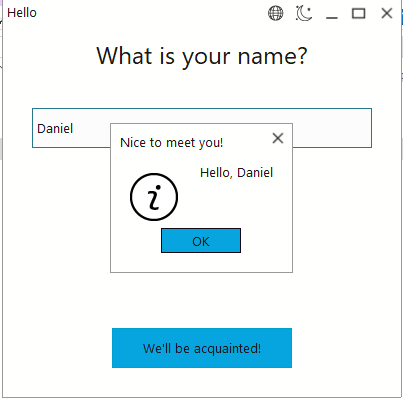
\includegraphics[width=0.8\linewidth]{test4}}
	\caption{Всплывающее окно}
	\label{msg:image}
\end{figure}

Функция: окно подтверждения.

Условия: нажата кнопка выхода из приложения.

Входные данные: событие нажатия кнопки мыши на кнопку закрытия.

Результат: появление окна закрытия (рисунок \ref{msg-y-n:image}).

\begin{figure}[H] % H - рисунок обязательно здесь, или переносится, оставляя пустоту
	\center{
\includegraphics[width=0.8\linewidth]{test15}}
	\caption{Окно подтверждения закрытия}
	\label{msg-y-n:image}
\end{figure}

Функция: подсказка.

Условия: наведение курсора мыши на иконку кнопки.

Входные данные: положение курсора, обработчик события подсказки.

Результат: появление подсказки под кнопкой (рисунок \ref{tip:image}).

\begin{figure}[H] % H - рисунок обязательно здесь, или переносится, оставляя пустоту
	\center{
\includegraphics[width=0.8\linewidth]{test14}}
	\caption{Подсказка}
	\label{tip:image}
\end{figure}

Функция: развернуть окно во весь экран.

Условия: нажата кнопка "<Развернуть">.

Входные данные: размер экрана, обработчик события кнопки "<Развернуть">, состояние окна.

Результат: окно развернулось на полный экран, изменился размер внутренних элементов окна. (рисунок \ref{fullscreen:image}).

\begin{figure}[H] % H - рисунок обязательно здесь, или переносится, оставляя пустоту
	\center{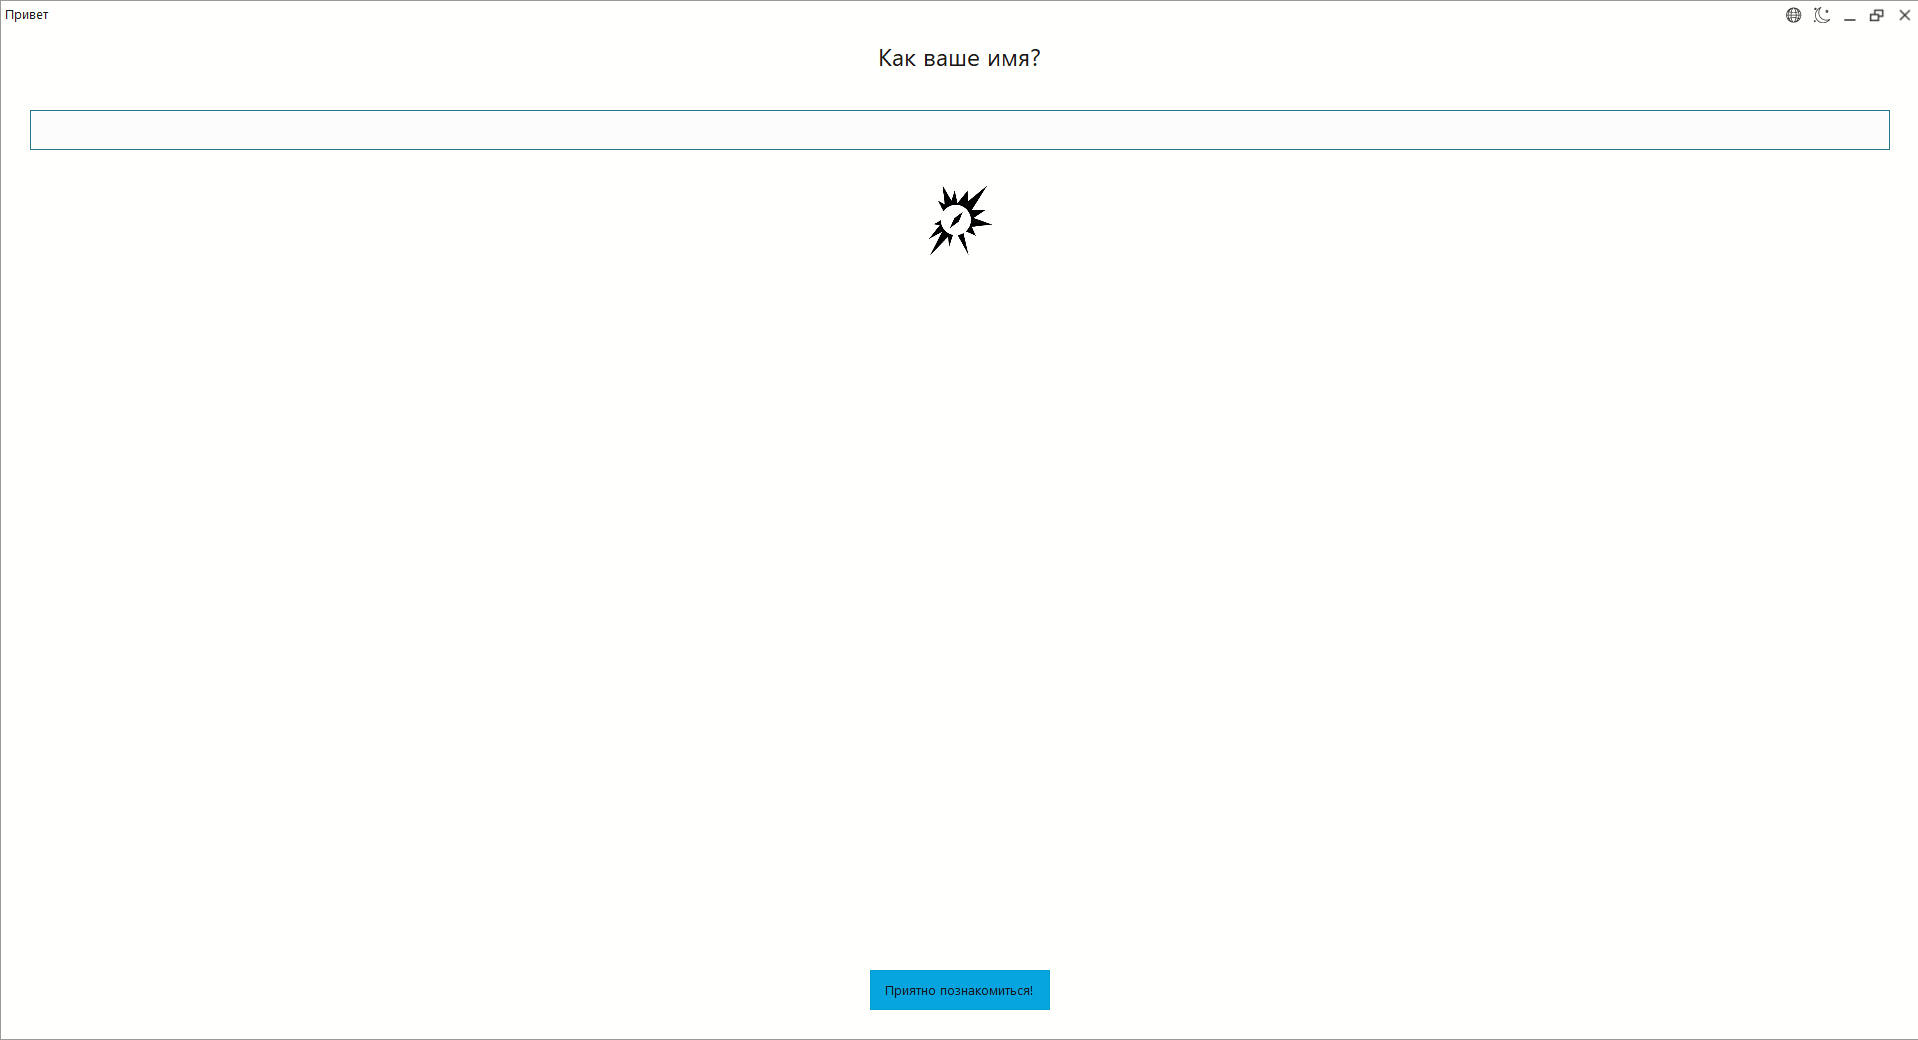
\includegraphics[width=0.8\linewidth]{test16}}
	\caption{Приложение, развернутое на полный экран}
	\label{fullscreen:image}
\end{figure}

Функция: ползунок.

Условия: изменено положение ползунка.

Входные данные: позиция ползунка, обработчик события ползунка.

Результат: на экране появилась координата х, в случае изменения положения горизонтального ползунка, и координата y при изменении положения вертикального ползунка.
. (рисунок \ref{scroll:image}).

\begin{figure}[H] % H - рисунок обязательно здесь, или переносится, оставляя пустоту
	\center{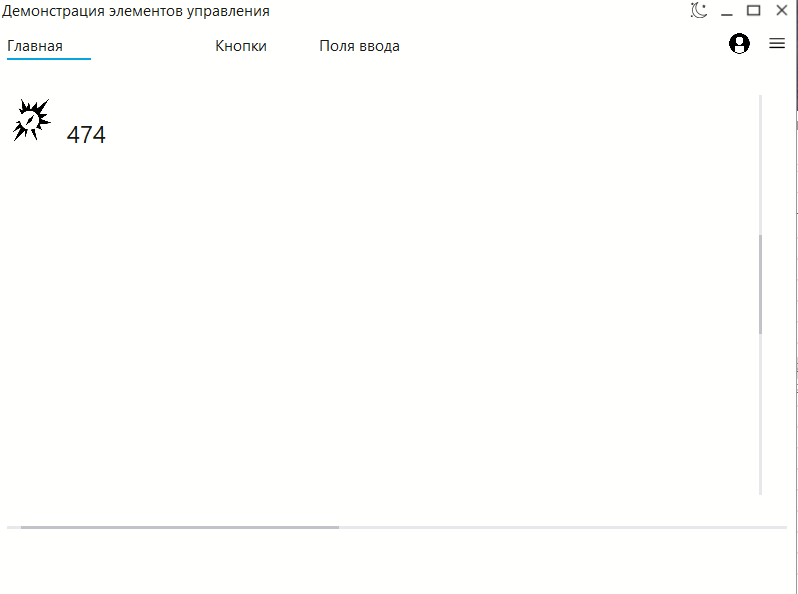
\includegraphics[width=0.8\linewidth]{test7}}
	\caption{Ползунок}
	\label{scroll:image}
\end{figure}

Функция: поле для ввода.

Условия: в поле для ввода введен текст.

Входные данные: фокус поля для ввода, обработчик события клавиатуры.

Результат: на экране появился текст.
. (рисунок \ref{input:image}).

\begin{figure}[H] % H - рисунок обязательно здесь, или переносится, оставляя пустоту
	\center{
\includegraphics[width=0.8\linewidth]{test17}}
	\caption{Поле для ввода}
	\label{input:image}
\end{figure}

Функция: нажатие кнопки.

Условия: нажатие кнопки мыши на кнопку.

Входные данные: событие нажатия кнопки мыши на кнопку, нажатая кнопка.

Результат: появилось текстовое сообщение о том какая кнопка нажата. (рисунок \ref{button:image}).

\begin{figure}[H] % H - рисунок обязательно здесь, или переносится, оставляя пустоту
	\center{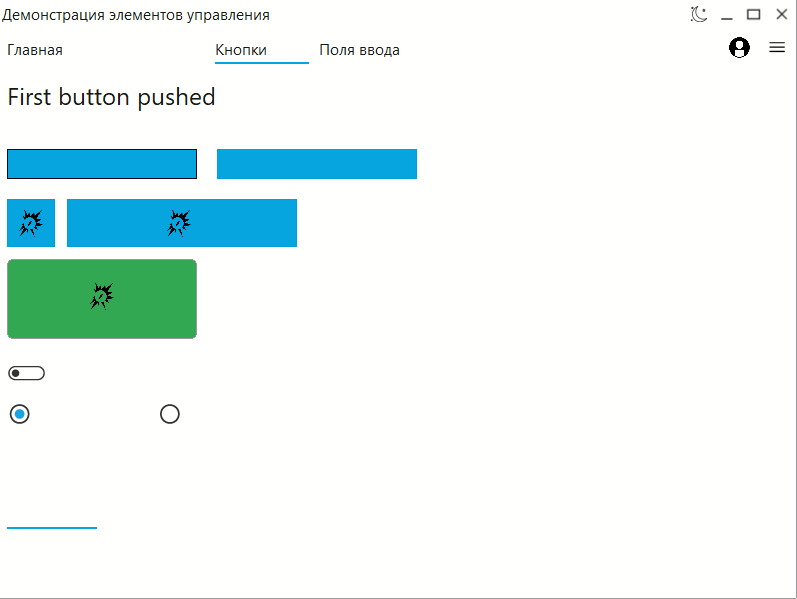
\includegraphics[width=0.8\linewidth]{test5}}
	\caption{Нажатие кнопки}
	\label{button:image}
\end{figure}

Функция: нажатие переключателя.

Условия: нажатие кнопки мыши на переключатель.

Входные данные: событие нажатия кнопки мыши на переключатель, нажатый переключатель.

Результат: появилось текстовое сообщение о том, что нажат переключатель. (рисунок \ref{switcher:image}).

\begin{figure}[H] % H - рисунок обязательно здесь, или переносится, оставляя пустоту
	\center{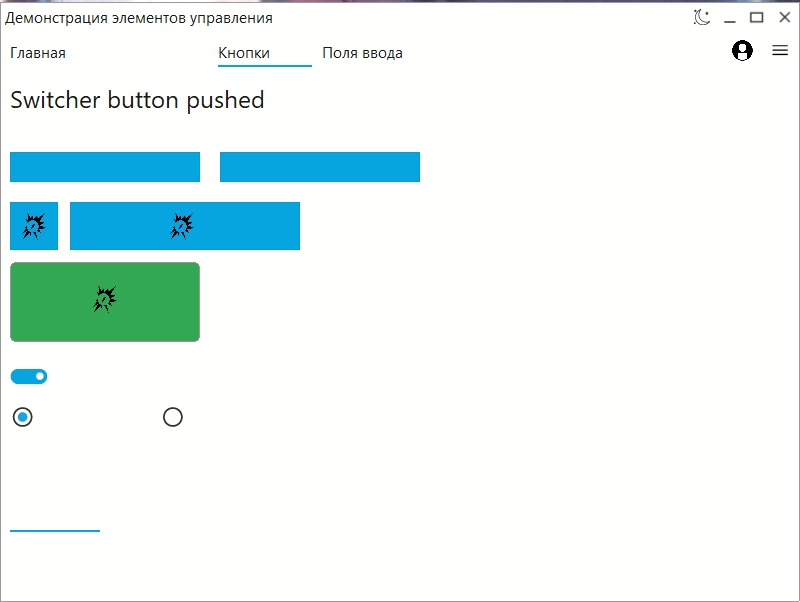
\includegraphics[width=0.8\linewidth]{test10}}
	\caption{Нажатие переключателя}
	\label{switcher:image}
\end{figure}

Функция: радиокнопка.

Условия: нажатие кнопки мыши на радиокнопку.

Входные данные: событие нажатия кнопки мыши на радиокнопку, нажатая радиокнопка.

Результат: появилось текстовое сообщение о том, что нажата радиокнопка. (рисунок \ref{radio:image}).

\begin{figure}[H] % H - рисунок обязательно здесь, или переносится, оставляя пустоту
	\center{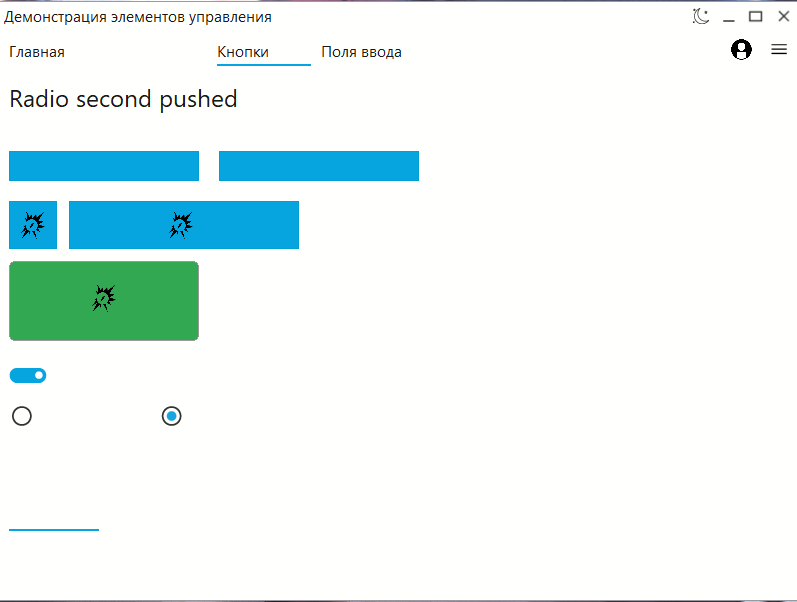
\includegraphics[width=0.8\linewidth]{test11}}
	\caption{Нажатие радиокнопки}
	\label{radio:image}
\end{figure}

Функция: смена страницы.

Условия: нажатие кнопки мыши на страницу.

Входные данные: событие нажатия кнопки мыши на страницу, нажатая страница.

Результат: появилось текстовое сообщение о том, что нажата страница. (рисунок \ref{sheet:image}).

\begin{figure}[H] % H - рисунок обязательно здесь, или переносится, оставляя пустоту
	\center{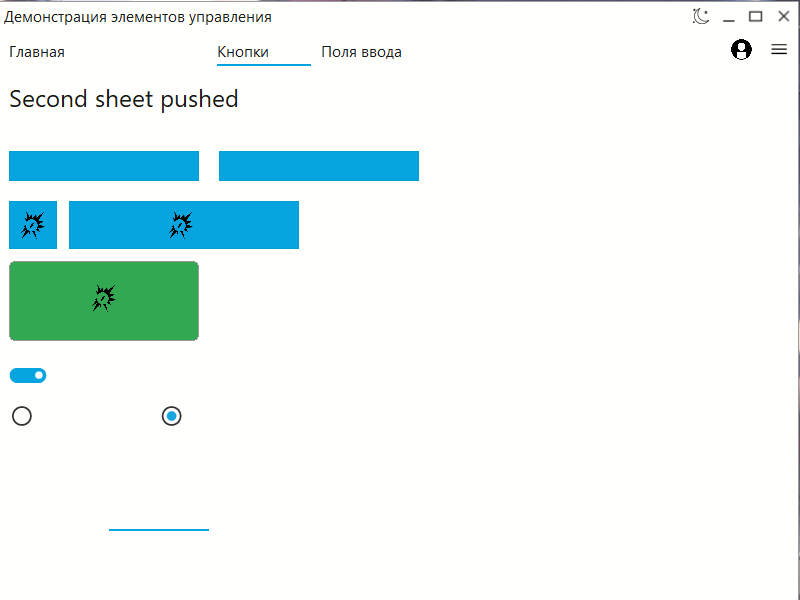
\includegraphics[width=0.8\linewidth]{test12}}
	\caption{Кнопка смены страницы}
	\label{sheet:image}
\end{figure}

Функция: ползунок настройки и полоса прогресса.

Условия: передвинут ползунок настройки.

Входные данные: положение ползунка настроек, обработчик событий.

Результат: при изменении положения ползунка настроек заполняется полоса прогресса. (рисунок \ref{slider:image}).

\begin{figure}[H] % H - рисунок обязательно здесь, или переносится, оставляя пустоту
	\center{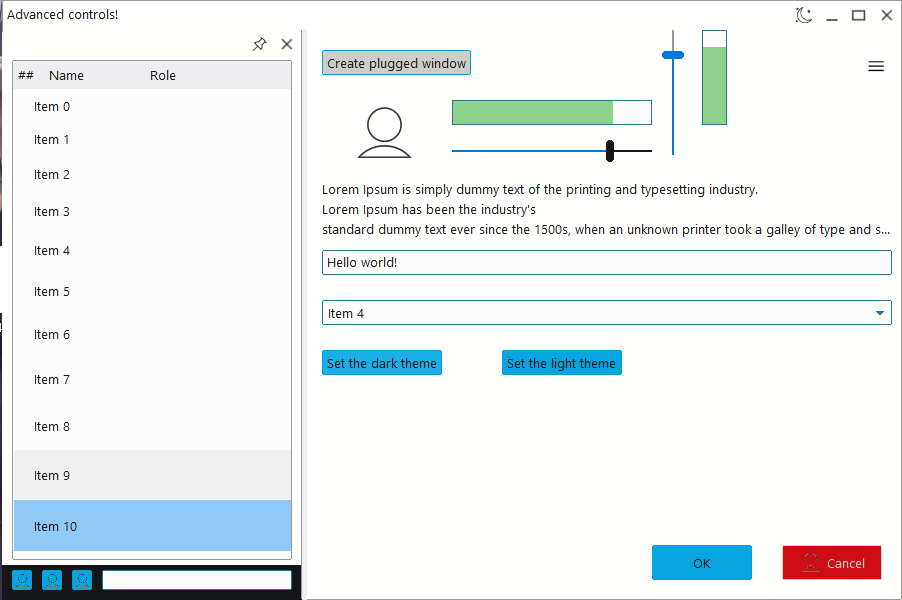
\includegraphics[width=0.8\linewidth]{test13}}
	\caption{Ползунок настройки и полоса прогресса}
	\label{slider:image}
\end{figure}

Функция: выпадающий список.

Условия: нажатие кнопки мыши на выпадающий список.

Входные данные: нажатие кнопки мыши на выпадающий список, обработчик события списка.

Результат: Раскрытие выпадающего списка. (рисунок \ref{list:image}).

\begin{figure}[H] % H - рисунок обязательно здесь, или переносится, оставляя пустоту
	\center{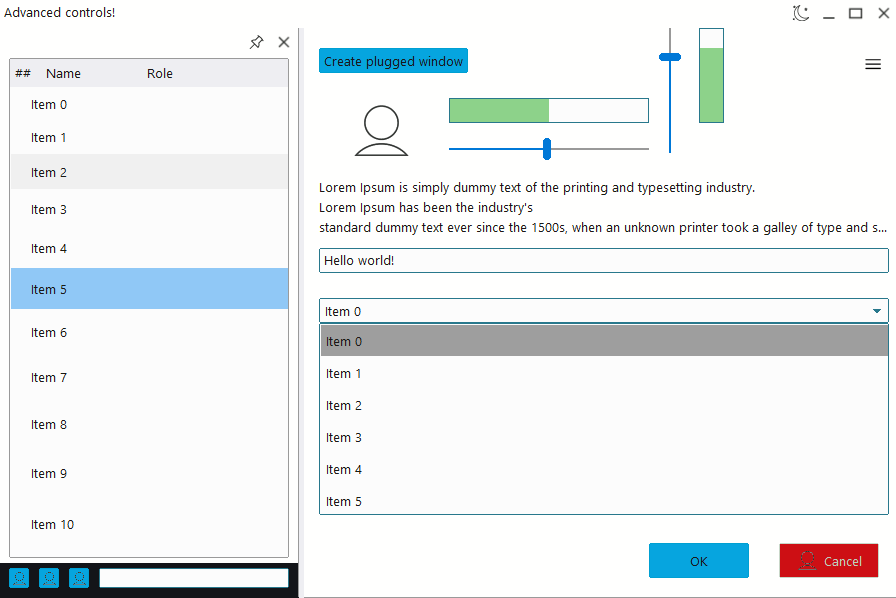
\includegraphics[width=0.8\linewidth]{test8}}
	\caption{Cписок}
	\label{list:image}
\end{figure}

Функция: Меню.

Условия: нажата кнопка настроек.

Входные данные: нажатие кнопки мыши на кнопку настроек, обработчик меню настроек.

Результат: на экране появилось меню. (рисунок \ref{menu:image}).

\begin{figure}[H] % H - рисунок обязательно здесь, или переносится, оставляя пустоту
	\center{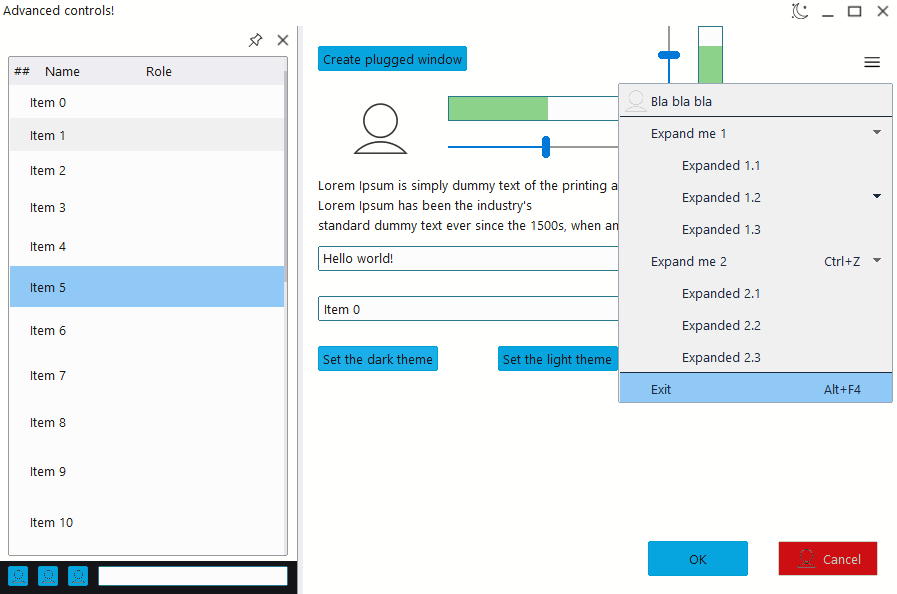
\includegraphics[width=0.8\linewidth]{test9}}
	\caption{Меню настроек}
	\label{menu:image}
\end{figure}

Функция: открепление окна.

Условия: нажатие кнопки мыши на кнопку открепления окна.

Входные данные: нажатие кнопки мыши на кнопку открепления окна, позиция окна, состояние окна, обработчик события.

Результат: появилось открепленное окно, которое можно двигать по экрану. (рисунок \ref{pin:image}).

\begin{figure}[H] % H - рисунок обязательно здесь, или переносится, оставляя пустоту
	\center{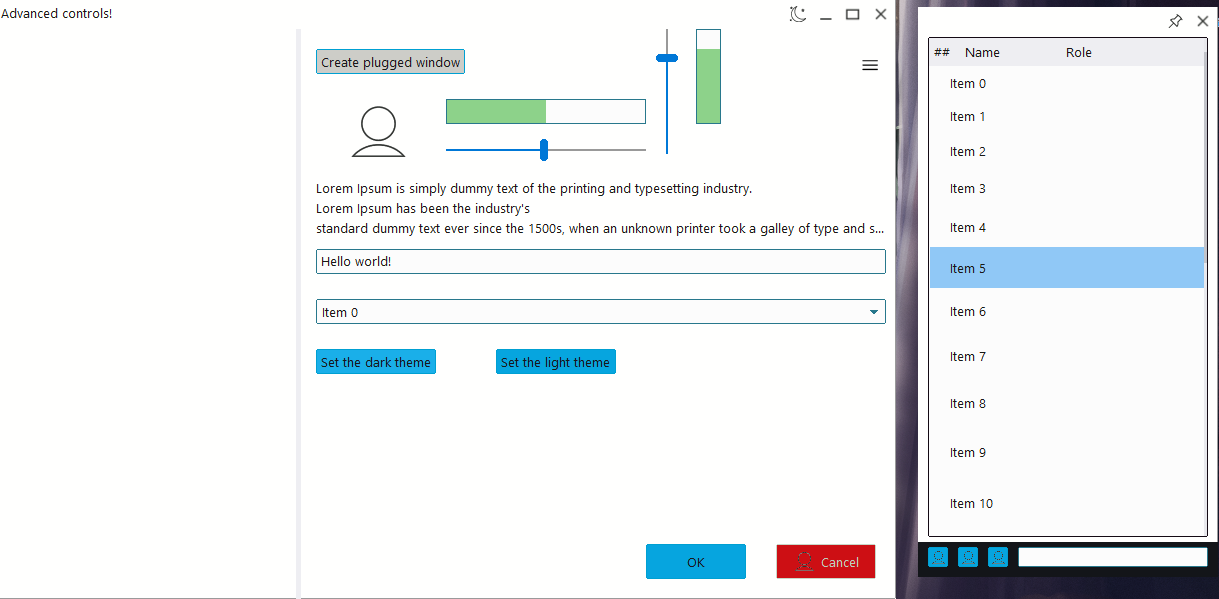
\includegraphics[width=0.8\linewidth]{test6}}
	\caption{Открепление окна}
	\label{pin:image}
\end{figure}
   \section*{ЗАКЛЮЧЕНИЕ}
\addcontentsline{toc}{section}{ЗАКЛЮЧЕНИЕ}

В ходе исследования было выявлено, что проектирование фреймворка для создания графического пользовательского интерфейса играет ключевую роль в обеспечении удобства использования программного продукта. Разработка такого фреймворка позволяет значительно упростить процесс создания интерфейсов, повысить их качество и снизить затраты на разработку. Отличительной особенностью успешного фреймворка является его гибкость, расширяемость и простота в использовании. Дальнейшее развитие в этом направлении сможет улучшить опыт пользователей и повысить эффективность разработки программных продуктов.

К особенностям данного фреймворка можно отнести встроенную поддержку локалей и цветовых тем на основе json-схем позволяет легко создавать впечатляющие многоязычные приложения с разнообразными цветовыми и визуальными темами. Еще одним приимуществом является небольшой средний размер двоичного кода, что позволило значительно уменьшить итоговый вес приложений. 

Основные результаты работы:

\begin{enumerate}
\item Проведен анализ предметной области. Выявлена необходимость использовать С++.
\item Разработана концептуальная модель фреймворка. Разработана модель данных системы. Определены требования к системе.
\item Cпроектирована программная система для создания графических пользовательских интерфейсов
\item Реализован и протестирован фреймворк. Проведено модульное и системное тестирование.
\end{enumerate}

Все требования, объявленные в техническом задании, были полностью реализованы, все задачи, поставленные в начале разработки проекта, были также решены.

Готовый рабочий проект представлен библиотекой. Фреймворк находится в публичном доступе, поскольку опубликован в сети Интернет.

Перспективой дальнейшей разработки является расширение списка поддерживаемых элементов управления и шаблонов программ.

}\fi
\addcontentsline{toc}{section}{СПИСОК ИСПОЛЬЗОВАННЫХ ИСТОЧНИКОВ}

\begin{thebibliography}{23}
	\bibitem{interface} Купер Алан. Интерфейс. Основы проектирования взаимодействия / А. Купер. – Санкт-Петербург: Питер, 2018. – 720 с. – ISBN 978-5-4461-0877-0. – Текст~: непосредственный.
	\bibitem{gui} Машин В. А. Проектирование и дизайн пользовательского интерфейса / В.А. Машин, А.К. Гультяев. – Санкт-Петербург: Корона Принт, 2010. – 352 с. – ISBN 978-5-7931-0814-0. – Текст~: непосредственный.
	\bibitem{framework} Gregory F. Rogers. Framework-Based Software Development in C++  / Gregory F. Rogers. – London: Pearson, 2008. – 400 с. – ISBN 978-0135333655. – Текст~: непосредственный.
	\bibitem{Qt} Прохоренок Николай. Qt 6. Разработка оконных приложений на C++ / Прохоренок Н.А. – Санкт-Петербург: БХВ, 2022. – 512 с. – ISBN 978-5-9775-1180-3. – Текст~: непосредственный.
	\bibitem{electron} Скотт Адам Д. Разработка на JavaScript. Построение кроссплатформенных приложений с помощью GraphQL, React, React Native и Electron / Скотт А. Д. – Санкт-Петербург: Питер, 2021. – 320 с. – ISBN 978-5-4461-1462-7. – Текст~: непосредственный.
	\bibitem{javafx} Прохоренок Николай. JavaFX / Прохоренок Н.А. – Санкт-Петербург: БХВ, 2019. – 768 с. – ISBN 978-5-9775-4072-8. – Текст~: непосредственный.
	\bibitem{gtk} Андрей Костельцов. GTK+. Разработка переносимых графических интерфейсов / Костельцов А.В. – Санкт-Петербург: БХВ, 2002. – 362 с. – ISBN 5-94157-161-5. – Текст~: непосредственный.
	\bibitem{wpf} Мак-Дональд Мэтью. WPF: Windows Presentation Foundation в .NET 4.5 с примерами на C{\#} 5.0 для профессионалов. / Мак-Дональд М. – Москва: Вильямс, 2013. – 1024 с. – ISBN 978-5-8459-1854-3. – Текст~: непосредственный.
	\bibitem{uml} Максимчук Р.А. UML для простых смертных /Максимчук  Р.А., Нейбург Э.Дж. – Москва: Лори, 2024. – 300 с. – ISBN 978-5-85582-434-6. – Текст~: непосредственный.
	\bibitem{gl} Гинсбург Дэн. OpenGL ES 3.0. Руководство разработчика / Гинсбург Д. – Санкт-Петербург: ДМК Пресс, 2015. – 449 с. – ISBN 978-5-97060-256-0. – Текст~: непосредственный.
	\bibitem{vulkan} Селлерс Грэхем. Vulkan. Руководство разработчика / Селлерс Г. – Санкт-Петербург: ДМК Пресс, 2017. – 394 с. – ISBN 978-5-97060-486-1. – Текст~: непосредственный.
    \bibitem{OOP} E. Balagurusamy. Object Oriented Programming With C++ / Balagurusamy E.  – New York Sity : McGraw-Hill Education (India) Pvt Limited, 2008 – 637 с. – ISBN 978-0070669079. – Текст~: непосредственный.
    \bibitem{c++} Paul Deitel C++ How to Program / Deitel P., Deitel H. – London: Pearson, 2016. – 1080 с. – ISBN 978-0134448237. – Текст~: непосредственный.
    \bibitem{recommendations} Мейерс Скотт. Эффективный и современный С++:42 рекомендации по использованию С++11 и С++14 / Мейерс С. – Москва~: Вильямс, 2019. – 304 с. – ISBN 978-5-907114-67-8. – Текст~: непосредственный.
	\bibitem{problems} Дьюхерст Стивен. Скользкие места С++. Как избежать проблем при проектировании и компиляции ваших программ / Дьюхерст С. – Москва~: ДМК Пресс, 2017. – 264 с. – ISBN 978-5-97060-475-5. – Текст~: непосредственный.
	\bibitem{beauty} Грегори Кейт. Красивый C++: 30 главных правил чистого, безопасного и быстрого кода / Кейт Г., Дэвидсон Дж. Г. – Санкт-Петербург~: Питер, 2023. – 368 с. – ISBN 978-5-4461-2272-1. – Текст~: непосредственный.
	\bibitem{creative} Спрол Антон. Думай как программист. Креативный подход к созданию кода. C++ версия / Спрол А. – Москва~: Эксмо, 2018. – 272 с. – ISBN 978-5-04-089838-1. – Текст~: непосредственный.
	\bibitem{boost} Полухин Антон. Разработка приложений на С++ с использованием Boost. Рецепты, упрощающие разработку вашего приложения / Полухин А. - Санкт-Петербург : ДМК Пресс, 2020. - 346 c. -ISBN 978-5-97060-868-5. – Текст~: непосредственный.
	\bibitem{chainik} Шилдт Герберт. C++ для начинающих / Шилдт Г. – Санкт-Петербург: Питер, 2024. – 608 с. – ISBN 978-5-4461-1821-2. – Текст~: непосредственный.
	\bibitem{practika} Евдокимов Петр. C++ на примерах. Практика, практика и только практика / Евдокимов П. В., Орленко П. А. – Санкт-Петербург: Наука и техника, 2022. – 288 с. – ISBN 978-5-94387-772-8. – Текст~: непосредственный.
	\bibitem{history} Страуструп Бьёрн. Дизайн и эволюция языка-С++. Второе издание / Страуструп Б. – Санкт-Петербург: ДМК Пресс, 2016. – 448 с. – ISBN 978-5-97060-419-9. – Текст~: непосредственный.
	\bibitem{visual} Пахомов Б.И. C/C++ и MS Visual C++ 2010 для начинающих / Пахомов Б.И. – Санкт-Петербург: БХВ, 2011. – 736 с. – ISBN 978-5-9775-0599-4. – Текст~: непосредственный.
	\bibitem{student} Побегайло А. П.  C/С++ для студента / Побегайло А. П. – Санкт-Петербург: БХВ, 2006. – 525 с. – ISBN 978-5-94157-647-1. – Текст~: непосредственный.
\end{thebibliography}

\ifВКР{\appendix{Представление графического материала}

Графический материал, выполненный на отдельных листах,
изображен на рисунках А.1--А.\arabic{числоПлакатов}.
\setcounter{числоПлакатов}{0}

\renewcommand{\thefigure}{А.\arabic{figure}} % шаблон номера для плакатов

\begin{landscape}

\begin{плакат}
    \includegraphics[width=0.82\linewidth]{плакат1.eps}
    \заголовок{Сведения о ВКРБ}
    \label{pl1:image}      
\end{плакат}

\begin{плакат}
    \includegraphics[width=0.82\linewidth]{плакат2.eps}
    \заголовок{Цель и задачи разработки}
    \label{pl2:image}      
\end{плакат}

\begin{плакат}
    \includegraphics[width=0.82\linewidth]{плакат3.eps}
    \заголовок{Концептуальная модель фреймворка}
    \label{pl3:image}      
\end{плакат}

\begin{плакат}
	\includegraphics[width=0.82\linewidth]{плакат4.eps}
	\заголовок{Интерфейс окна}
	\label{pl4:image}      
\end{плакат}

\begin{плакат}
    \includegraphics[width=0.82\linewidth]{плакат5.eps}
    \заголовок{Варианты использования}
    \label{pl5:image}      
\end{плакат}

\begin{плакат}
	\includegraphics[width=0.82\linewidth]{плакат6.eps}
	\заголовок{Схема обмена данных}
	\label{p16:image}      
\end{плакат}

\begin{плакат}
	\includegraphics[width=0.82\linewidth]{плакат7.eps}
	\заголовок{Тестирование}
	\label{pl7:image}      
\end{плакат}

\begin{плакат}
	\includegraphics[width=0.82\linewidth]{плакат8.eps}
	\заголовок{Заключение}
	\label{pl8:image}      
\end{плакат}

\end{landscape}
}\fi
\ifПрактика{}\else{\appendix{Фрагменты исходного кода программы}

framework.cpp
\lstinputlisting[language=C++, frame=none]{code/src/framework/framework.cpp}

window.cpp
\lstinputlisting[language=C++, frame=none]{code/src/window/window.cpp}

graphic.cpp
\lstinputlisting[language=C++, frame=none]{code/src/graphic/graphic.cpp}

locale.cpp
\lstinputlisting[language=C++, frame=none]{code/src/locale/locale.cpp}

theme.cpp
\lstinputlisting[language=C++, frame=none]{code/src/theme/theme.cpp}

i{\_}control.hpp
\lstinputlisting[language=C++, frame=none]{code/include/wui/control/i_control.hpp}

example.cpp
\lstinputlisting[language=C++, frame=none]{code/hw.cpp}

\ifВКР{
\newpage
\addcontentsline{toc}{section}{На отдельных листах (CD-RW в прикрепленном конверте)}
\begin{center}
\textbf{Место для диска}
\end{center}
}\fi
}\fi
\end{document}
